\documentclass[11pt, a4paper]{article}
\usepackage{tmh}
\usepackage{bbm}
\renewcommand{\labelenumi}{\roman{enumi}}
\renewcommand{\phi}{\varphi}

\renewcommand{\P}{\mathbb{P}}
\newcommand{\E}{\mathbb{E}}
\newcommand{\T}{\mathbb{T}}
\newcommand{\Z}{\mathbb{Z}}
\newcommand{\F}{\mathcal{F}}
\newcommand{\Dt}{\Delta t}
\newcommand{\Dv}{\Delta v}
\newcommand{\Dx}{\Delta x}
\newcommand{\dx}{\dif x}
\newcommand{\dt}{\dif t}
\renewcommand{\familydefault}{\sfdefault}
\usepackage[scaled]{helvet}
\setlength{\parindent}{0em}
\setlength{\parskip}{1em}
\usepackage{showkeys}

\title{{\huge Numerical Methods for an Interacting Particle System}}
\author{Thomas M. Hodgson\\ \vspace{0.5cm} Maxwell Institute Graduate School}
\date{\today}
\newcommand\testname{Acknowledgements}
\newenvironment{acknowledge}
{\renewcommand\abstractname{\testname}\begin{abstract}}
    {\end{abstract}}

\begin{document}
	\maketitle
    \thispagestyle{empty}
	\newpage
	\tableofcontents
	\listoffigures
	\newpage
    \begin{abstract}
        +++ +++
    \end{abstract}
    \begin{acknowledge}
        +++Seb, Desvages +++
    \end{acknowledge}
      \newpage 
	\section{Introduction}\label{sec:introduction}
        Many natural phenomena arise from the interaction of many agents. Very complex behaviour can emerge from simple interaction rules -- a classic example is the murmurations seen in flocks of starlings. Here wonderful patterns emerge even though each starling interacts with only its 6-7 nearest neighbours \cite{Ballerini08}. Shoaling fish also exhibit similar flocking behaviour. This behaviour provides a social group for the species, as well as providing increased protection from predators and increased chance of mating. It also allows mass migration to occur. Understanding and developing models for these systems is an area of great interest, interacting particles are present from the microscopic scale (mammal cells, bacteria, even electromagnetism), all the way to large mammals communicating across oceans. The goal is to approximate the complexity present in these systems using as few simple rules as possible.

Broadly speaking, there are two closely-linked approaches to modelling particle systems \cite{Berdahl17}. The first is a particle- or agent-based model, in which every agent is modelled as a discrete object updating its behaviour based on other agents in the system. The second is a kinetic model, commonly seen in statistical mechanics for large numbers of molecules. Here there are no particles, we instead consider the density of particles at a given time and configuration of the system. One of the classic studies into collective motion was the work of Vicsek et al. \cite{Vicsek95} in which what is now known as the Vicsek model was proposed.

\subsection{Vicsek Model}
In the Vicsek model, particles align based on the average direction of the velocities all the other particles in the system. That is, at time $t+\Dt$ the position, $x^{i,N}$ of the $i^{\text{th}}$ particle is given by
\[ x^{i,N}(t+\Dt) =     x^{i,N}(t) + v^{i,N}(t)\Dt\]
where $v^{i,N}(t)$ is the velocity of the particle at time $t$. All particles have the same magnitude of velocity, and the direction is given by an angle $\theta$ where
\[\theta(t+\Dt) = \langle \theta(t)\rangle_r + \Delta \theta.\]
Here, $\langle \theta(t)\rangle_r$ denotes the average direction of the velocities of all particles within a distance $r$ of the $i^{\text{th}}$ particle. The term $\Delta \theta$ is a random variable uniformly distributed on $[-\eta/2,\eta/2]$.

This simple system was shown to have a critical point at which the motion of the particles changed from unordered to flocking behaviour, before transitioning to completely ordered motion. 

The original Vicsek model is limited. It cannot incorporate different types of interaction between the particles and the interaction suddenly disappears as a particle moves beyond a distance $r$ from another particle. Other models, such as the Cucker-Smale model \cite{Cucker07}, adapt the model so that the magnitude of the velocity is not fixed, and the interaction is a much smoother function. Both the Vicsek and Cucker-Smale models are very theoretical in their approach. A more traditional biological approach is presented by Couzin et al. \cite{Couzin02}. Here they considered three different regions around each particle: the zones of repulsion, orientation and attraction. The goal here was to create a more natural model that incorporates animals desire to maintain a fixed distance between each other -- preventing collisions or dispersion. A 'field of perception' can also be incorporated, reflecting that most biological agents do not have $360^{\circ}$ vision.

In this report we focus on the model introduced in \cite{Butta2019}. This model is similar to the Vicsek model in that particles align based on other particles velocities, however it is much more flexible in how the interaction is described. In Section \ref{sec:model} the particle model, along with its associated kinetic model, is introduced and described term by term. In Section \ref{sec:dynamics}, the dynamics of the model are investigated. In Section \ref{sec:numericalmethods}, the numerical methods required to approximate these models numerically are presented, before being applied in Section \ref{sec:application}. Avenues for possible future work are given in Section \ref{sec:discussion}.

       
	\section{The Model}\label{sec:model}
        		We here introduce the model of Butt\`a, Flandoli, Ottobre and Zegarlinski \cite{Butta2019}. This is a Vicsek-type continuum model for an interacting particle system. There are three key parts to this model that together create interaction and ordered motion: a herding function, denoted $G$; an averaging function, denoted $M$; and an interaction function, $\phi$. Each will be described before the full model is introduced. Throughout, we will be considering the phase space distribution function $f_t(x,v)$, where $(x,v) \in \T \times \R$ and $t \in \R$ with $\T \cong \R \backslash \Z \cong S^1$ denoting the unit one-dimensional torus. The distribution function represents the density of particles at time $t$ at a given point in phase space $(x,v)$.
		
		The interaction function, $\phi: \T \to \R $ acts on the smallest scale, between individual points. It is smooth and satisfies the following:
		\begin{align}\label{eq:phi}
			\phi(x) \geq \epsilon >0, && \phi(x) = \phi(-x), &&& \int_{\T} \phi(x) \dif x = 1.
		\end{align}
		These are quite natural ways to describe an interaction. The first means that all points interact with each other to some degree. The second requires symmetry when interacting, and finally the function must have unit integral -- this is only for simplicity and could in fact be any value, so long as it is finite. For example, we may take $\phi \equiv 1$. This will satisfy the above requirements and corresponds to all points interacting an equal amount, regardless of position on the torus. This will create space-homogeneity, which we will return to later.
		
		The function $M:\R \to \R$ takes a weighted average of the interactions across the space.	
		\[ 
			M(t,x) = \frac{\int_{\T}\int_{\R}f_t(y,w)\phi(x-y)w\dif w \dif y}{\int_{\T}\int_{\R}f_t(y,w)\phi(x-y)\dif w \dif y}
		\]
		The interaction function provides the weighting. Note the argument of  $\phi$ is the distance between two points in space and also that $M$ depends on $f_t$. The denominator is required in the corresponding particle model to prevent the size of the group of particles from having an effect on the dynamics. It can be thought of as a normaliser.
		
		Finally, the herding function $G:\R \to \R$ is chosen such that
		\begin{align*}
			&G(u)=-G(-u),&& {\begin{cases}
								G(u)>u & \text{ if } 0< u <1\\
								G(u)<u & \text{ if } u > 1
				   		   \end{cases}}.
		\end{align*}
		We shall consider three forms of $G$.
		\begin{enumerate}
			\item Step:
			\[
				G(u) = \frac{1+\beta \mathrm{sgn}(u)}{1+\beta}, \qquad \beta > 0	
			\]
			This is the usual choice in the biological literature, with \(\beta = \frac{1}{2}\). It is differentiable everywhere with $G'(u) = \frac{1}{1+\beta}$, except at $u=0$. This discontinuity makes analysis more difficult.
			\item Smooth:
			\[
				G(u) = \frac{\arctan(u)}{\arctan(1)}
			\]
			Here we get a much smoother curve that is everywhere differentiable. However the gradient isn't very steep and there is no way to control the shape of the curve.
			\item Sigmoid:
			\[
				G(u) = \frac{2}{1+\mathrm{e}^{-\alpha u}} - 1 , \qquad \alpha >0
			\]
			The sigmoid herding function provides a middle ground between the previous two. It is smooth, but can be made as sharp as required by adjusting the parameter $\alpha$. However note that it only satisfies second requirement above in the limit as $\alpha \to \infty$ as the function is bounded above by 1.
		\end{enumerate}
		During the analysis, we will use the smooth herding function for its amenability. The role of $G$ is to herd the mean velocity towards a fixed value -- in this case plus or minus one. How it does so will become clearer when we discuss the dynamics of the model.
        \begin{figure}
            \centering
            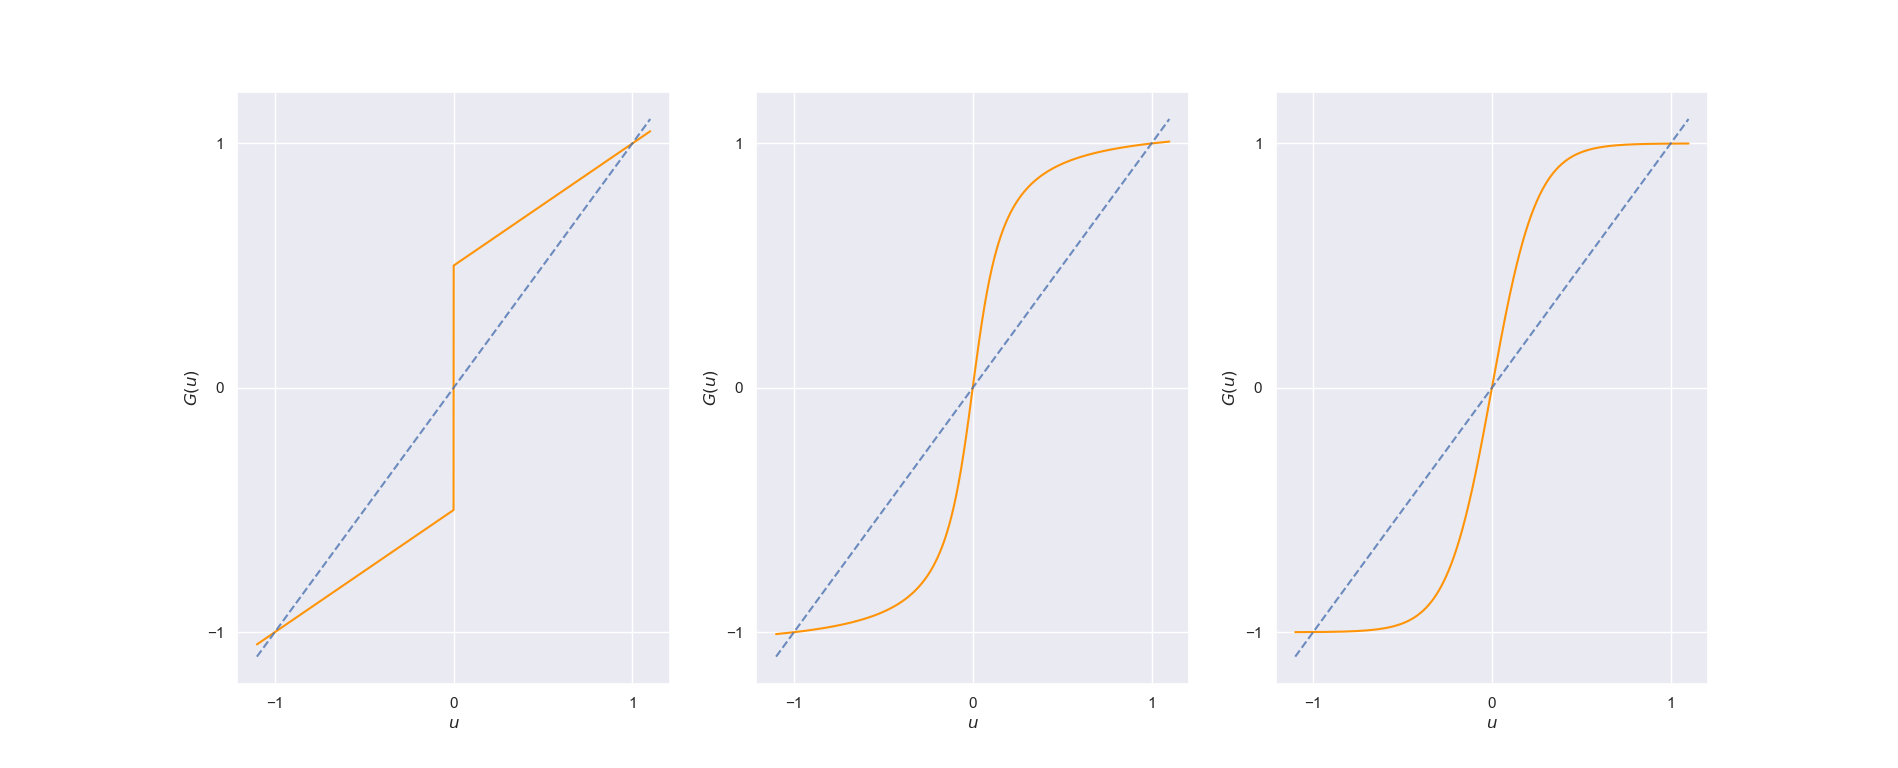
\includegraphics[width=\linewidth]{Figures/herdingfunctions}
            \caption{Step, smooth and sigmoid herding functions, with the dashed line $y=x$ for reference}
            \label{fig:herdingfunctions}
        \end{figure}
		We now have all the necessary ingredients to give the full continuum model. The evolution of the distribution is described by
		\begin{equation}\label{eq:fullPDE}
			\partial_t f_t(x,v) = -v\partial_x f_t(x,v)  +\partial_v v f_t(x,v) - \partial_v \left[ G(M(t,x))f_t(x,v)\right] + \sigma \partial_{vv}f_t(x,v),
		\end{equation}
		where $\sigma > 0$ is a constant describing the rate of diffusion. At its heart, this is just an advection-diffusion equation. The first term illustrates the movement around the torus, the second describes a damping effect and the fourth gives a diffusive effect in velocity. The third term is where the interest lies as it contains all the information on interaction and herding.
		
        
	\section{Dynamics}\label{sec:dynamics}
        		To better understand the dynamics of \eqref{eq:fullPDE}, first let $G\equiv0$. This removes any interaction between particles and the equation becomes
		\begin{equation}\label{eq:OUFPE}
			\partial_t f_t(x,v) = -v\partial_x f_t(x,v) +\partial_v vf_t(x,v) + \sigma \partial_{vv}f_t(x,v).
		\end{equation}
		This is the Fokker-Planck equation for the following system:
		\begin{equation}\label{eq:2dOU}\begin{cases}
			\dif x_t = v_t\dif t\\
			\dif v_t = -v_t\dif t + \sqrt{2\sigma} \dif W_t. 
		\end{cases}	\end{equation}
		Here, $W_t$ is a standard one-dimensional Wiener process. We recognise this as overdamped Langevin dynamics, and so we can exactly calculate the unique invariant measure. To do so it is necessary to solve $\partial_t \rho_t = 0$, that is, when is the density not changing in time. The evolution in $v$ is described by an Ornstein-Uhlenbeck process so it is known that the unique stationary distribution is Gaussian with mean $1$ and variance $\sigma$. The position $x$ depends only on $v$ with no noise. There is no reason to assume any sort of mean reverting behaviour and expect the density to spread out uniformly on the torus. A guess at the solution would then be $\rho (x,v) = \frac{1}{2\pi}\exp(\frac{-v^2}{2})$, with some normalising constant. Notice that this equation does not depend on $x$. By substitution into the stationary Fokker-Planck equation, this is indeed a solution.
        
        Similarly, when $G\not\equiv 0$ the density $f_t(x,v)$ of \eqref{eq:fullPDE} is the Fokker-Planck equation of the two dimensional SDE,
		    \begin{equation}\label{eq:McKV}\begin{cases}
		    \dif x_t = v_t\dif t\\
		    \dif v_t = \left[G(M(t,x_t))-v_t\right] \dif t + \sqrt{2\sigma} \dif W_t. 
			\end{cases} \qquad  (x_t,v_t) \in \T \times \R
			\end{equation}
		This is a McKean-Vlasov equation as the function $M(t,x_t)$ conceals a dependence on the law of the process. 
        \[
            M(t,x) = \frac{\E\left[ v'_t \phi(x-x'_t)\right]}{\E\left[\phi(x-x'_t)\right]}
        \]
        The pair $(x'_t,v'_t)$ is a random variable equal in distribution to $(x_t,v_t)$. This representation of $M(t,x)$ is the same as the one given previously, however in this setting it is natural to use expectation notation over integrals. To illustrate the necessity of introducing another random variable, albeit one that is equal in law, consider the case when the interaction function is the indicator on the interval $[-b,b]$, $\phi(x) = \mathbbm{1}_{[-b,b]}(x)$. This does not meet the requirements in Section \ref{sec:model}, in particular it is neither strictly positive nor does it have unit integral. 
        \begin{align*}
            M(t,x) &=  \frac{\int_{\T}\int_{\R}f_t(y,w)\phi(x-y)w\dif w \dif y}{\int_{\T}\int_{\R}f_t(y,w)\phi(x-y)\dif w \dif y}\\
            &=  \frac{\int_{\T}\int_{\R}f_t(y,w) \mathbbm{1}_{[-b,b]}w\dif w \dif y}{\int_{\T}\int_{\R}f_t(y,w) \mathbbm{1}_{[-b,b]}\dif w \dif y}\\
            &= \frac{\E\left[ v'_t \mathbbm{1}_{[-b,b]}\right]}{\P(x' \in \left[x-b,x+b\right])}\\
            &= \E\left[ v'_t|x' \in [x-b,x+b] \right]
        \end{align*}
        It makes no sense to consider $\P(x \in [x-b,x+b])$ as it is always equal to one so the auxiliary variable $(x'_t,v'_t)$ is used. +++More detail?+++ This calculation also illustrates how $\phi$ describes the interaction or `where to look' while $M$ acts as a average velocity of the points `within range'. The transport term, $\partial_v\left( \left[ v-G(M(t,x))\right]f_t(x,v)\right)$ then acts to change the velocity towards the local average given by $M$. It is in this sense that $G$ is the herding function `herding' the system towards a common velocity.
        
        The McKean-Vlasov representation of the system is also the weak limit of an $N$-body particle system described by
        \begin{equation}\label{eq:fullparticle}\begin{cases}
            \dif x^{i,N}_t = v^{i,N}_t\dif t\\
            \dif v^{i,N}_t = -v^{i,N}_t\dif t + G\left(\frac{\frac{1}{N}\sum_{j=1}^N \phi(x_t^{i,N} - x_t^{j,N})v^{j,N}_t  }{\frac{1}{N}\sum_{j=1}^N \phi(x_t^{i,N} - x_t^{j,N})}\right)\dif t + \sqrt{2\sigma} \dif W^i_t 
            \end{cases}, \qquad  i = 1,\dots,N.
        \end{equation}
        This gives another view of the full system \eqref{eq:fullPDE}, and one that is particularly amenable to analysis. It also allows a more intuitive view of the system -- rather than thinking of how a density changes over time, we can think of particles moving around a torus and interacting according to $\phi$.
        
        \subsection{Invariant Measures under Space Homogeneity}
        Thus far, we have found the invariant measure for only the rather uninteresting case when $G \equiv 0$. To progress further, we must simplify the system. One way to do this is to impose that the density does not depend on the position in space and set $\phi \equiv 1$. The weighted local average velocity $M$ becomes neither local nor weighted. In the particle system, this means that each particle interacts with every other particle, irrespective of the distance between them. Indeed,
        \begin{align*}
            M(t,x) =&  \frac{\int_{\T}\int_{\R}f_t(y,w)\phi(x-y)w\dif w \dif y}{\int_{\T}\int_{\R}f_t(y,w)\phi(x-y)\dif w \dif y}\\
            =&  \frac{\int_{\T}\int_{\R}f_t(y,w)w\dif w \dif y}{\int_{\T}\int_{\R}f_t(y,w)\dif w \dif y}\\
            =& \int_{\T}\int_{\R}f_t(y,w)w\dif w \dif y\\
            :=& \langle w \rangle_{f_t}.
        \end{align*}
        So the weighted local average velocity is just the average of the distribution $f_t(v)$ or equivalently, the average velocity of all particles in the system. The evolution is then described by
        \begin{equation}\label{eq:spacehomPDE}
            \partial_t f_t(v) = \partial_v vf_t(v) - \partial_v G(\langle w \rangle_{f_t})f_t(v) + \sigma \partial_{vv} f_t(v).
        \end{equation}
        The above problem's well-posedness can be shown as follows. Let
        \[
            h_t(v) = f_t(u),\text{ where } u = v + \int_0^t G(\langle w\rangle_{f_t}) \dif s.
        \]
        To find an equation that $h_t(v)$ solves, we use the chain rule.
        \begin{align*}
            \partial_t f_t(u) &= \partial_t f_t(u) +  G(\langle w\rangle_{f_t})\partial_v f_t(u) && \text{as   } \pd{g}{v} = 1, \pd{g}{t} = G((\langle w\rangle_{f_t})\\
            &=\partial_v vf_t(u) - \partial_v G(\langle w \rangle_{f_t})f_t(u) + \sigma \partial_{vv} f_t(u) + G(\langle w\rangle_{f_t})\partial_v f_t(u) &&\text{as  } f_t \text{ solves } \eqref{eq:spacehomPDE}\\
            &=\partial_v vh_t(v) + \sigma \partial_{vv} h_t(v) , \qquad h_0(v) =f_0(v).
        \end{align*}
        So $h_t$ solves the Fokker-Planck equation for the one-dimensional Ornstein-Uhlenbeck process which is well posed +++cite+++. Therefore the solution $f_t(v)$ of \eqref{eq:spacehomPDE} exists and is unique given initial data. To find invariant measures of this evolution, set the transient term to zero and solve the remaining PDE, which can be written in gradient form. First note that if $G\equiv 0$, this system for $f_t$ is the same as that for $h_t$, and so has a unique invariant measure $\mathcal{N}(0,\sigma)$. When the herding function is non-zero, other measures are also stationary as we will now show. For brevity, we omit the dependence on $v$ of $f$ and write $\langle w \rangle_{f_t} = M_1$. The latter is natural as it denotes the first moment of the distribution.
        \begin{align*}
            &\partial_v\left[(-G(M_1) +v) f + \sigma \partial_v f \right] = 0\\
            \implies& (-G(M_1) +v) f + \sigma \partial_v f = C_1
        \end{align*}
        This ODE is solvable and gives 
        \[
            f(v) = C_2\exp\left(\frac{2G(M_1)v - v^2}{2\sigma} \right). 
        \]
        Applying the constraint $\int_\R f(w)\dif w = 1$ gives $C_2 = \exp(-G^2(M_1))/\sqrt{2\pi\sigma}$. +++note here this is a Gaussian with mean $G(M_1)$? Immediately implies that $M_1 = G(M_1)$ without need for integration +++ Furthermore, from the definition of space average,
        \begin{align*}
            M_1 :=& \int_\R wf(w) \dif w\\ 
            =& \int_\R \frac{w\exp(-G^2(M_1))}{\sqrt{2\pi\sigma}} \exp\left(\frac{2G(M_1)v - v^2}{2\sigma} \right)\\ 
            =& \int_\R \frac{w}{\sqrt{2\pi\sigma}} \exp\left(\frac{ - (v-G(M_1))^2}{2\sigma} \right)\\
            =& G(M_1)
        \end{align*}
        Using the smoothed version of the herding function from Section \ref{sec:model} gives $G(M_1) = 0, \pm 1$. Substituting this into our expression for $f$ gives three invariant measures:
        \begin{align*}
            \rho_0 &= \frac{1}{\sqrt{2\pi\sigma}}\exp\left(-\frac{v^2}{2\sigma} \right), && \rho_{\pm} = \frac{1}{\sqrt{2\pi\sigma}}\exp\left(-\frac{(v\pm 1)^2}{2\sigma}\right).
        \end{align*}
        These are Gaussian densities with mean $0, \pm 1$ and variance $\sigma$.
        
        We have found three invariant measures for the evolution \eqref{eq:spacehomPDE}, however whether the system will converge to these distributions given initial data remains to be settled. In the space homogeneous case it is possible to close equations on the moments of the distribution. Let $M_n = \int_\R v^n f_t(v) \dif v$ denote the n$^\text{th}$ moment of the distribution $f_t(v)$. Then
        \begin{align*}
            \partial_t M_n(t) &= \int_{\R}v^n \partial_t  f_t(v) \dif v\\
            &= - \int_{\R}v^n \partial_v G(M_1)f_t(v) \dif v + \int_{\R}v^n \partial_v vf_t(v) \dif v + \sigma \int_{\R}v^n \partial_vv f_t(v) \dif v,
        \end{align*}
        as $f_t$ solves the space-homogeneous PDE \eqref{eq:spacehomPDE}. Using integration by parts and simplifying gives, for the first three moments,
        \begin{align*}
            \dot{M}_0 &= 0,\\
            \dot{M}_1 &= G(M_1) - M_1,\\
            \dot{M}_2 &= 2\lbrack M_1G(M_1) - M_2 + \sigma\rbrack.
        \end{align*}
        The first tells us there is no change in the zeroth moment over time, that is probability is conserved. The equation for the first moment has equilibria at -1, 0 and 1 for the smoothed choice of $G$. Figure +++ref+++ shows the phase plane diagram for this ODE. It shows that given any initial data with positive average velocity, the first moment will converge to one. By symmetry, the same is true for negative initial data, the mean will converge towards negative one. It also shows that mean zero is an unstable equilibrium -- a slight perturbation will move the system from random movement to ordered motion.
        \begin{figure}
            \centering
            %\includegraphics[width=0.7\linewidth]{}
            \caption{Phase plane of the first  +++(and second?)+++ moment ODE}
            \label{fig:M1phase}
        \end{figure}
        To find the convergence of the variance, we must look at the difference between the second moment and the square of the first.
        \begin{align*}
            \od{}{t}\lbrack M_2 - M_1^2\rbrack &= \dot{M}_2 - 2M_1\dot{M}_1\\
            &= 2\lbrack G(M_1)M_1 - M_2 +\sigma\rbrack - 2M_1\lbrack G(M_1) - M_1\rbrack\\
            &= -2M_2 +2\sigma + 2M_1^2\\
            &= 2\lbrack M_2 - M_1^2 -\sigma\rbrack             
        \end{align*}
        Solving this ODE gives $M_2-M_1^2 = \sigma +(\sigma_0-\sigma)\mathrm{e}^{-2t}$, where $\sigma_0$ is the variance of the initial data $f_0$. Then as $t \to \infty$, it can be seen that the system forgets its initial data and tends towards a distribution with variance $\sigma$.
        
        The equations on the moments have shown that the system indeed converges to a measure with mean $\pm 1$ and variance $\sigma$ however this is not sufficient to conclude that they are Gaussian. To do so requires closing equations on all the cumulants of the distribution. It can be shown that these vanish for all cumulants of order greater than three and so the system indeed converges towards the invariant measures found by solving the space-homogeneous PDE \eqref{eq:spacehomPDE}. This means that irrespective of initial data, we expect all particles to move on average in the same direction with the same velocity -- a phenomenon known as unconditional flocking. The only exception is when the initial data has mean zero. In this case the system will converge to the Gaussian with mean zero, corresponding to disordered motion. +++not a great explanation+++
        
        The dynamics of the space-homogeneous system have thus been fully characterised analytically. We will now turn our attention to the particle model in this case.
    \subsubsection{Particle System Dynamics}\label{sec:particledynamics}
        As the particle system approximates the McKean-Vlasov SDE, whose density solves the PDE \eqref{eq:spacehomPDE}, one would expect that it behaves in entirely the same way. This is in fact not the case, as we will now show. Consider the particle system \eqref{eq:fullparticle} in the space-homogeneous case,
        \begin{equation}\label{eq:homparticle}
            \dif v^{i,N}_t = G\left(\frac{1}{N}\sum_{j=1}^n v^{j,N}_t\right)\dif t-v^{i,N}_t \dif t + \sqrt{2\sigma} \dif W^i_t
        \end{equation}
        It has been shown for the kinetic model that the invariant measures have mean zero and $\pm 1$ when we consider a smoothed herding function. Here we will show that the space-homogeneous particle model only admits invariant measures with mean zero for any herding function satisfying the earlier requirements in Section \ref{sec:model}, before finding analytic forms for the functions we will be using. First note that in the case of no interaction, that is $G\equiv 0$, the dynamics are governed by an Ornstein-Uhlenbeck process leading to a unique stationary distribution with mean zero. This is in agreement with the solution to the PDE under no interaction in Section \ref{sec:dynamics}. When $G\not\equiv 0$, the invariant distribution still always has mean zero, unlike what we have seen for the space-homogeneous kinetic model. Given that we wish to find the behaviour of the mean velocity, it would be pertinent to find an equation that it solves. To this end, let $m_t = \frac{1}{N}\sum_{j=1}^N v^{j,N}_t$. Summing the system across $i$ gives an equation for $m_t$:
        \[
            \dif m_t = \lbrack -m_t + G(m_t)\rbrack \dif t +\sqrt{2\sigma}\dif W_t
        \]
        Let $V(x) = \frac{x^2}{2} + \tilde{V}(x)$, where $-\tilde{V}'(x) = G(x)$ so that $-V'(x) = -x + G(x)$. The aim here is to find a function $V$ such that the equation for $m_t$ resembles the Langevin equation. The existence and uniqueness of the invariant measure will then follow from standard theory for the Langevin equation and its associated Fokker-Planck equation. Thus
        \begin{equation}\label{eq:meanSDE}
            \dif m_t = -V'(m_t)\dif t + \sqrt{2\sigma}\dif W_t.
        \end{equation}    
        By definition, $\tilde{V}(x) = - \int_{-\infty}^x G(u) \dif u$. As $G$ is bounded, $\tilde{V}(x)$ grows at most linearly. This means $V(x) \to \infty$ as $|x|\to \infty$, $V$ is a well-defined potential well and $\mathrm{e}^{-V(x)}$ is integrable. Hence \eqref{eq:meanSDE} admits a unique invariant measure, $\rho(x) = \mathcal{Z}^{-1}\mathrm{e}^{-V(x)}$ with $\mathcal{Z}$ a normalising constant.
        
        What can we say about this invariant measure? Recall the only restrictions placed on $G$ in Section \ref{sec:model} were firstly $G$ must be odd, that is $G(u)=-G(-u)$, and secondly,
        \[
            \begin{cases}
            G(u)>u & \text{if } 0<u<1,\\ 
            G(u)<u &  \text{if } u>1.
            \end{cases}
        \]
         
        If $G$ is odd, $\tilde{V}(x)$ is an even function, so $V(x)$ is also an even function. Then the mean of the invariant distribution $\rho$ is
        \[
            \mathbb{E}_{\rho}[m] = \mathcal{Z}^{-1}\int_{\mathbb{R}} m \mathrm{e}^{-V(m)}\dif m = 0,
        \]
        as this is the integral of an odd function. The behaviour of the particle system is then fundamentally different to that of its corresponding kinetic model, despite weakly converging to the McKean-Vlasov SDE \eqref{eq:McKV} whose density solves the PDE \eqref{eq:spacehomPDE}. This is in fact a well-known problem in the area of mean field equations +++cite+++. 
        
    The behaviour of the particle system here is not wholly unexpected -- the change in velocity is inherently random. To see how this affects the invariant measure, first recall the case when $G\equiv 0$, in which the particle system is the Ornstein-Uhlenbeck process and the kinetic model is its corresponding Fokker-Planck equation \eqref{eq:OUFPE}. Here, the particle moves in a potential well with a parabolic shape with a minima at zero. When $G\not\equiv 0$, the particles move within a double-well potential. For the choices of the herding function described here, this well will have minima at -1, 0 and 1\footnote{This is not quite true for any sigmoid $G$ in which $\alpha$ is not large enough.}. Moving deterministically,as the evolution described by the kinetic model is, the particles must settle in one of the two wells leading to a system with mean 1, 0 or -1. Under random movement however, there is a chance that the Wiener process forces the particle to jump over the potential barrier and into the other well. If this happens to enough particles, the remaining particles will also make the jump due to the effect of the herding function. We thus expect, for a finite number of particles, the motion to switch randomly between having average velocity positive one and negative one leading to the invariant measure having mean zero. This switching of mean velocity is known as metastability -- the Gaussian invariant measures for the PDE are only metastable in the particle model. We emphasise again that the dynamics under the kinetic model are fully deterministic and as such no switch of stability is possible. +++Dynkin's formula? Calc on exp time to switch?+++
        
        \begin{figure}
            \centering
        %    \includegraphics[width=0.7\linewidth]{" "}
            \caption{Particles in wells. Parabolic (OU) and Double Well showing jump between}
            \label{fig:particlewells}
        \end{figure}
        
        The method used above to characterise the mean of the distribution gives all that is required to calculate closed forms of the invariant measure. Table \ref{tab:spaceparticleinv} gives expressions for the three herding functions given in Section \ref{sec:model}.
        \begin{table}
        \centering
        \begin{tabular}{|c|c|c|}
            \hline 
            & & \\[-0.5em] 
            & Herding Function & Invariant Measure \\[10pt]
            \hline
            & & \\[-0.5em] 
            Step & $\frac{1+\mathrm{sgn}(u)}{2}$ & +++not correct, not double well or normalised+++ $\exp\left(\frac{|v|}{2}\right)$ \\[10pt]
            \hline 
            & & \\[-0.5em]
            Smooth &$\frac{\arctan(u)}{\arctan(1)}$  & $\frac{1}{(v^2+1)^{\frac{2}{\pi}}} \exp\left( -\frac{v^2}{2}+\frac{4}{\pi}v\mathrm{arctan}(v)\right)$ \\[10pt]
            \hline 
            & & \\[-0.5em]
            Sigmoid & $\frac{2}{1+\mathrm{e}^{-\alpha u}} - 1$ & $ \mathcal{Z}^{-1}(\mathrm{e}^{\alpha v}+1)^{\frac{2}{\alpha}}\exp\left(-\frac{v^2}{2} - v\right)$ \\[10pt]
            \hline 
        \end{tabular}
        \caption[Space-Homogeneous Particle Densities]{Normalised densities for the space-homogeneous particle model \eqref{eq:homparticle} with different herding functions}
        \label{tab:spaceparticleinv}
        \end{table}
    
        +++Convergence to invariant measure? Depends on metastability, rate of switching between wells +++
     
        \begin{figure}[h!]
            \centering
            %\includegraphics[width=0.7\linewidth]{}
            \caption[Potential Wells]{Potential Wells for the invariant measure of the space-homogeneous particle system for various herding functions}
            \label{fig:spacehomparticlemeasure}
        \end{figure}
        +++Full particle model invariant measure?+++\\
        In the space-homogeneous case, the analysis above gives a full picture of the dynamics of both the particle model and the kinetic model. However, the full system \eqref{eq:fullPDE} is much harder to analyse. It can be shown that the invariant measures for \eqref{eq:spacehomPDE} are also invariant, however it cannot be shown that they are the only ones. In particular, it can not be expressed in a gradient form like it could be in the space-homogeneous case. The aim now is to exploit our understanding of the space-homogeneous case to develop robust numerical techniques to learn more about the full system.
        
   	\section{Numerical Methods}\label{sec:numericalmethods}
        The analysis presented so far has been able to fully characterise the behaviour of the space-homogeneous kinetic model. However, it is unable to describe the dynamics of the full space-inhomogeneous model. It has been shown that the space-homogeneous model possesses only three invariant measures and converges to one of them dependent on the sign of the mean of the initial data. The full model also has these invariant measures, however it is not proven whether these are all of them or not. That is, the full model may have stationary distributions which are not homogeneous in space. By utilising numerical methods, we can relax some of the restrictions which the analysis requires. The goal is to show that for some choice of initial data and interaction function, the particle system will have a stationary distribution that isn't uniform in space. At its most basic, this could be two clusters of particles moving on the same direction diametrically opposite each other. The system will still converge in velocity to the values predicted by the homogeneous model, but spatial heterogeneity will remain. While this may be the case for the particle system, we conjecture that such behaviour will not occur in the kinetic model.

The aim is to be able to accurately simulate the dynamics of both the space-inhomogeneous PDE +++ref+++ and the corresponding interacting particle system. The latter is relatively simple to simulate using techniques for SDEs. However, we have shown analytically that the particle system does not have the same invariant measures as the continuum model, or indeed its McKean-Vlasov equation. The kinetic model is more difficult as it contains both advective and diffusive terms. We begin this section with a presentation of numerical methods for SDEs before reviewing methods for advection-type and diffusion-type equations, following the treatment of Hundsdorfer and Verwer \cite{Hundsdorfer2007} as well as Morton and Meyers \cite{Morton2005}.

Mirroring the approach in the analysis, we will develop the techniques required first for the space-homogeneous system with no interaction, before adding further levels of complexity. Doing so allows the rigorous testing of any schemes developed as analytic solutions are available. Throughout this section it is recommended to follow along with the supplementary Jupyter notebook available at: 
 %\url{https://github.com/Tom271/Whales} +++Change name+++
Every figure within this report was produced using the notebook and its accompanying source code.

\subsection{Particle Systems}\label{sec:homparticlesystem}
Simulating particle systems requires the numerical solution of coupled SDEs. The standard method for this is the Euler-Maruyama (EM) method, which can be seen as the stochastic analogue of Euler's method. Our motivating example here will be the Ornstein-Uhlenbeck process\footnote{This is also the overdamped Langevin equation}. 
\begin{equation}
\dif x_t = - x_t \dif t + \sigma \dif W_t
\end{equation}
This is exactly the same evolution as that which drives the space-homogeneous particle system \eqref{eq:homparticle}, with no interaction between particles, and so provides the ideal starting point. It describes the motion of a damped particle moving randomly within a potential well as illustrated in Section \ref{sec:particledynamics}. Applying the EM method to the above equation gives:
\[ x_{n+1} = x_n -  x_n\Dt + \sqrt{2\sigma\Dt}Z_n,  \]
where $Z_n$ is a standard normal random variable. This discretisation is very quick to compute, and has strong order $\frac{1}{2}$ \cite{Higham01}. This gives us a method of finding the stationary distribution: simulate many particles for a long time. Eventually, the density of the particles will be approximately the stationary distribution of the system. In this case it is in fact not even necessary to simulate many particles -- if the system is allowed to evolve for long enough, one particle will suffice as there is no interaction between particles and the scheme is ergodic. The particle system will be an excellent metric by which to test the schemes developed for the continuum models. One drawback however will be the presence of only one invariant measure, as was shown analytically in Section \ref{sec:particledynamics} and will be shown numerically in Section \ref{sec:homparticles}.
\begin{figure}
    \centering
    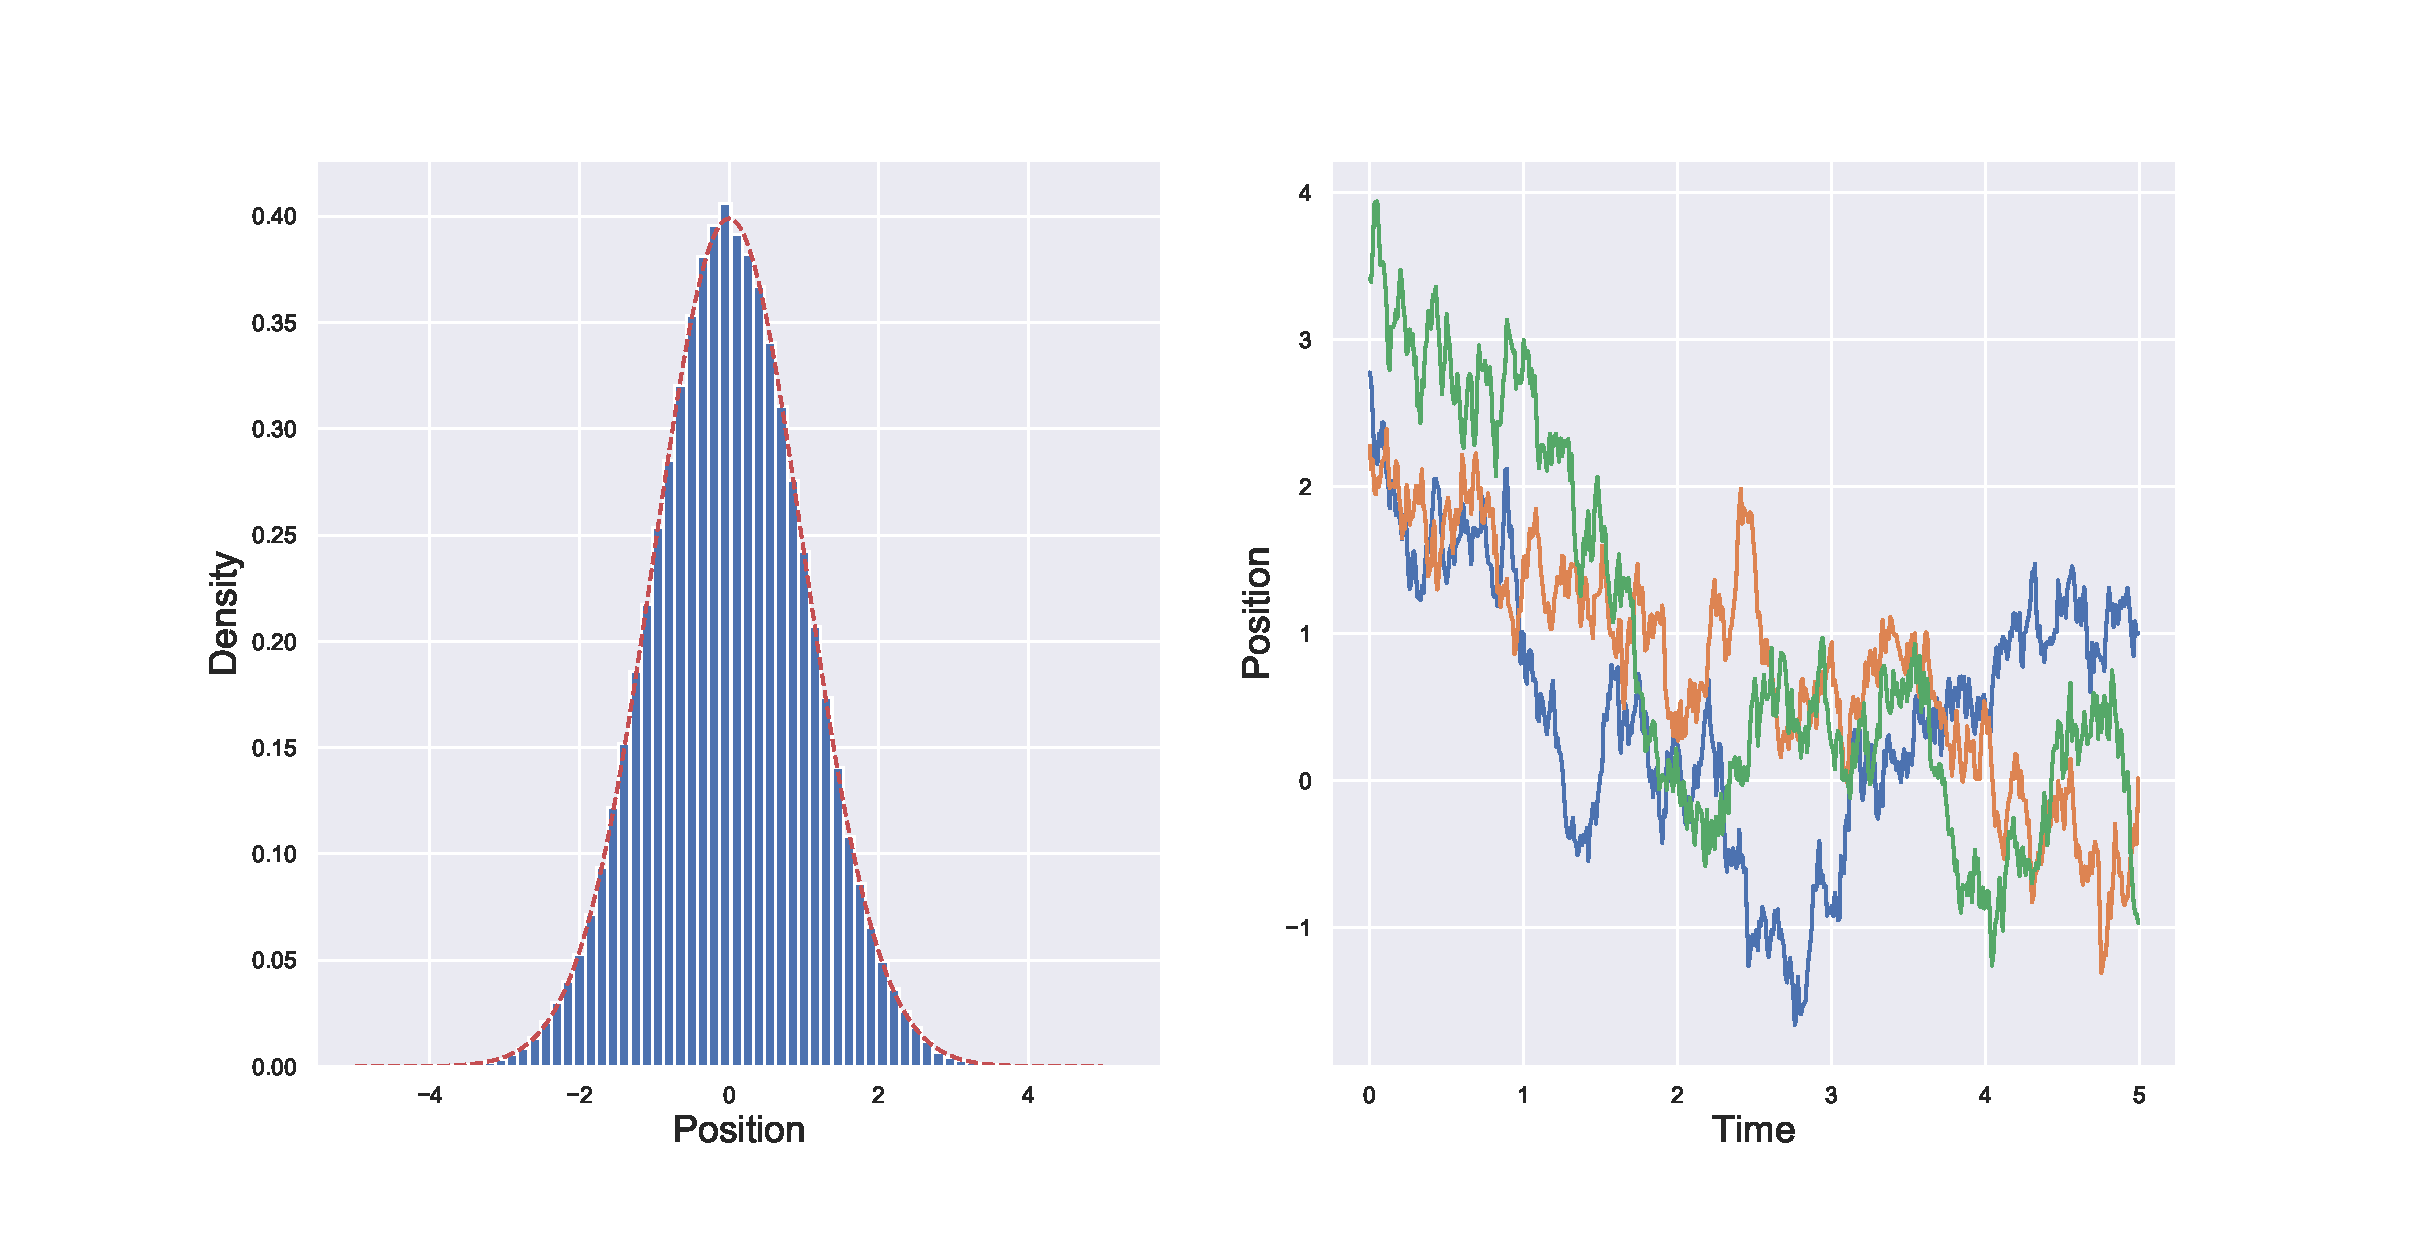
\includegraphics[width=\linewidth]{Figures/OUparticletraj}
    \caption{Histogram of positions of 1000 particles after 100s with $\sigma = 1$, and positions of 5 particles over time. +++conv in moments?+++}
    \label{fig:ouparticletraj}
\end{figure}

\subsection{Diffusion Equations}
As a prototypical example of a diffusion equation, consider the heat equation in one dimension given by 
\begin{equation}\label{eq:heat}
\begin{cases}
    \partial_t u(t,x) = \sigma\partial_{xx} u(t,x),&\sigma >0\\
        u(0,x) = u_0(x),  &t\in\R^+, x\in\R,
\end{cases}
\end{equation}
To solve this numerically, we must truncate the domain in both time and space. To do this, a region is chosen where we expect most of the mass to be throughout the time of interest. Here, we truncate to \(x \in [-L,L], t \in [0,T]\) for some \(L>0\) and a finite time horizon \(T\). Doing so requires a boundary condition to be enforced. A natural choice for this equation is a zero Dirichlet condition, \(u(t,L) = u(t,-L) = 0\). As long as \(L\) is chosen large enough, the heat which spreads beyond this limit is negligible -- this will however be a source of error. To mitigate this, one could compare the difference between analytic solutions (where available) on the full real line and the truncated domain, then choosing $L$ accordingly. In general, boundary conditions are determined by the phenomenon being modelled. The problem geometry may naturally suggest conditions, or they may be enforced by numerical constraints as in this case. We must also discretise in space and time, to create a mesh covering \(\left[0,T\right] \times \left[-L,L\right]\). Let \(\lbrace x_j\rbrace_{j=0}^J\) partition the space equally such that \(x_0 = -L, x_J=L\) and \(x_j-x_{j-1} = \Delta x\) for all \(j\). Similarly, let \(\lbrace t_n\rbrace_{n=0}^N\) partition \(\left[0,T\right]\) in such a way that \(t_0=0, t_N =T\) and \(t_n-t_{n-1} = \Delta t\). The parameters \(\Delta x, \Delta t\) are the space step and time step respectively. We thus have a discretised description of the continuum that we can implement. 

\subsubsection*{Forward Time Centred Space}
The aim is to solve the equation approximately on this grid. We shall denote approximate solutions by capital letters, that is \(u(x_j,t_n) \approx U_j^n\). How can we approximate the solution? We must approximate each term in the equation separately. First the time derivative, or transient term can be approximated using the definition of the derivative. Recall
\[
\od{u}{t} = \lim_{\Delta t \to 0}\frac{u(t+\Dt) - u(t)}{\Dt}.
\]
We can then approximate the time derivative for fixed $x$ by simply taking \(\Dt\) small. Doing so leads to the forward difference approximation
\[
\partial_t u(t_n,x_j) \approx \frac{U^{n+1}_j- U^n_j}{\Dt}.
\]
\begin{figure}
    \centering
    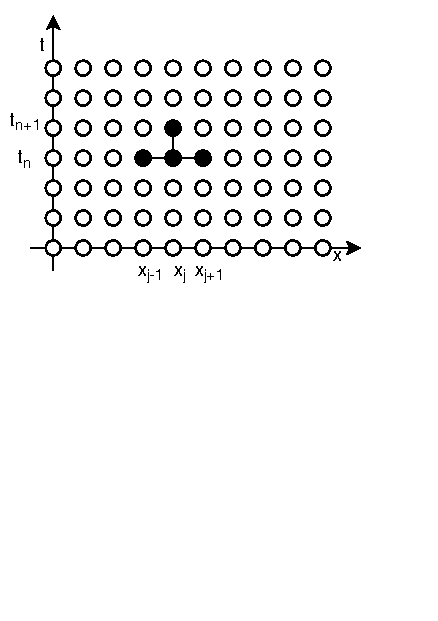
\includegraphics[width=0.5\linewidth, trim={0 5cm 0 0}]{Figures/FTCS}
    \caption[FTCS stencil]{Points used in the FTCS method}
    \label{fig:FTCSmesh}
\end{figure}


Now for the diffusion term, the most obvious approximation is to apply the forward difference scheme twice.
\begin{align*}
\partial_{xx} u(t_n,x_j) &\approx \partial_x \left(\frac{U^n_{j+1}- U^n_j}{\Dx}\right)\\
&=  \left(\frac{\partial_x U^n_{j+1} - \partial_x U^n_j}{\Dx}\right)\\
&\approx \frac{U^n_{j+1} - 2U^n_{j} + U^n_{j-1}}{(\Dx)^2}
\end{align*}
This is sufficient to give a first approximation to \eqref{eq:heat}.
\begin{align}\label{eq:FTCSheat}
\frac{U^{n+1}_j- U^n_j}{\Dt} &= \sigma \frac{U^n_{j+1} - 2U^n_{j} + U^n_{j-1}}{(\Dx)^2}\\
U^{n+1}_j &= U^n_j +  \frac{\sigma\Dt}{(\Dx)^2}\lbrack U^n_{j+1} - 2U^n_{j} + U^n_{j-1}\rbrack 
\end{align}
This is the Forward Time Centred Space (FTCS) method, a fully explicit scheme which means that we can write the next time step solely in terms of known values. We now have a method for approximating the true solution. When developing any numerical scheme, three properties need to be considered: stability, consistency and convergence. These concepts will be developed further below. Heuristically, a scheme is unstable if certain mesh spacings cause rapid growth in solutions -- a blow-up. A method is consistent if the error it makes in each step tends to zero as the size of the step tends to zero. Finally, a scheme is convergent if the approximate solution tends towards the true solution for any point in space and time. 

The heat equation \eqref{eq:heat} can be solved by separation of variables, giving the solution as a Fourier series. If the initial data is a single Fourier mode, the solution is
\begin{align*}
&u(t,x) = \mathrm{e}^{-\sigma(2\pi k)^2 t} \phi_k(x), && \phi_k(x) = \mathrm{e}^{2\pi i k x} \text{ for } k \in \mathbb{Z}.
\end{align*} 
If we assume our approximate solution is a Fourier mode, a criterion for stability will emerge.
\begin{align}
&U^n_j = \lambda^n \mathrm{e}^{ik(j\Dx)}, \qquad k \in \mathbb{Z} \label{eq:fouriermode}\\
\implies &U^{n+1}_j = \lambda U^n_j, \qquad U^n_{j\pm 1} = \mathrm{e}^{\pm ik\Dx}U^n_j \notag \\
\end{align}
Clearly if $|\lambda|>1$, the solution will be unstable. Substituting this into the finite difference scheme \eqref{eq:FTCSheat} gives
\begin{equation}\label{eq:FTCSlambda}
\lambda = 1 - 4\mu \sin^2\left(\frac{k\Dx}{2}\right), \qquad \text{ with } \mu = \frac{\sigma \Dt}{(\Dx)^2},
\end{equation}
and so,
\[
U^n_j = \left(1 - 4\mu \sin^2\left(\frac{k\Dx}{2}\right)\right)^n\mathrm{e}^{ikj\Dx}.
\]
Looking at \eqref{eq:fouriermode}, as $n \to \infty$, the numerical solution will grow unless $|\lambda|\leq 1$. If  $|\lambda|\leq 1$, the solution will decay with higher modes being damped quicker. This is what we expect from our analytic knowledge of the heat equation. The restriction on the mesh spacing thus arises from \eqref{eq:FTCSlambda}, 
\begin{align*}
-1 \leq \lambda \leq 1 \implies  \mu = \frac{\sigma \Dt}{(\Dx) ^2} \leq \frac{1}{2}
\end{align*}
This is not ideal: if more accuracy is required in the solution we can refine the space mesh, however in doing so the time step must also be shortened to maintain stability and the computational effort quickly increases.


The error made in each time step is the local truncation error, $R$, of the scheme. The local truncation error is the residual obtained by substituting the exact solution $u(t,x)$ into the discretisation. Performing a Taylor expansion around $t = n\Dt$ gives
\begin{align*}
&u^{n+1}_j = u^n_j + \Dt \partial_t u^n_j + \frac{1}{2}(\Dt)^2 \partial_{tt} u^n_j + \mathcal{O}(\Dt^3)\\
\implies& \frac{u^{n+1}_j - u^n_j}{\Dt}= \partial_t u^n_j + \frac{1}{2}\Dt \partial_{tt} u^n_j + \mathcal{O}(\Dt^2).
\end{align*}

And similarly around $x=j\Dx$,
\begin{align*}
&u^n_{j+1}=  u^n_j + \Dx \partial_x u^n_j + \frac{1}{2}(\Dx)^2 \partial_{xx} u^n_j + \frac{1}{3!}(\Dx)^3 \partial_{xxx} u^n_j + \frac{1}{4!}(\Dx)^4 \partial_{xxxx} u^n_j +  \mathcal{O}(\Dx^5)\\
\implies& \frac{u^n_{j+1} -2  u^n_j + u^n_{j-1}}{\Dx^2}  = \partial_{xx}u^n_j + (\Dx)^2u_{xxx} + \mathcal{O}(\Dx^3).
\end{align*}  
The local truncation error is then
\begin{align*}
&R^n_j = \underbrace{\partial_t u^n_j - \sigma \partial_{xx}u^n_j}_{=0} +\mathcal{O}(\Dt)+ \mathcal{O}(\Dx^2)\\
\implies& R^n_j = \mathcal{O}(\Dt)+\mathcal{O}(\Dx^2).
\end{align*}
The first two terms are zero as $u$ is solves the heat equation. The explicit scheme \eqref{eq:FTCSheat} is then first order in time and second order in space. 

\begin{figure}
    \centering
    \begin{minipage}[b]{0.49\textwidth}
        \centering
        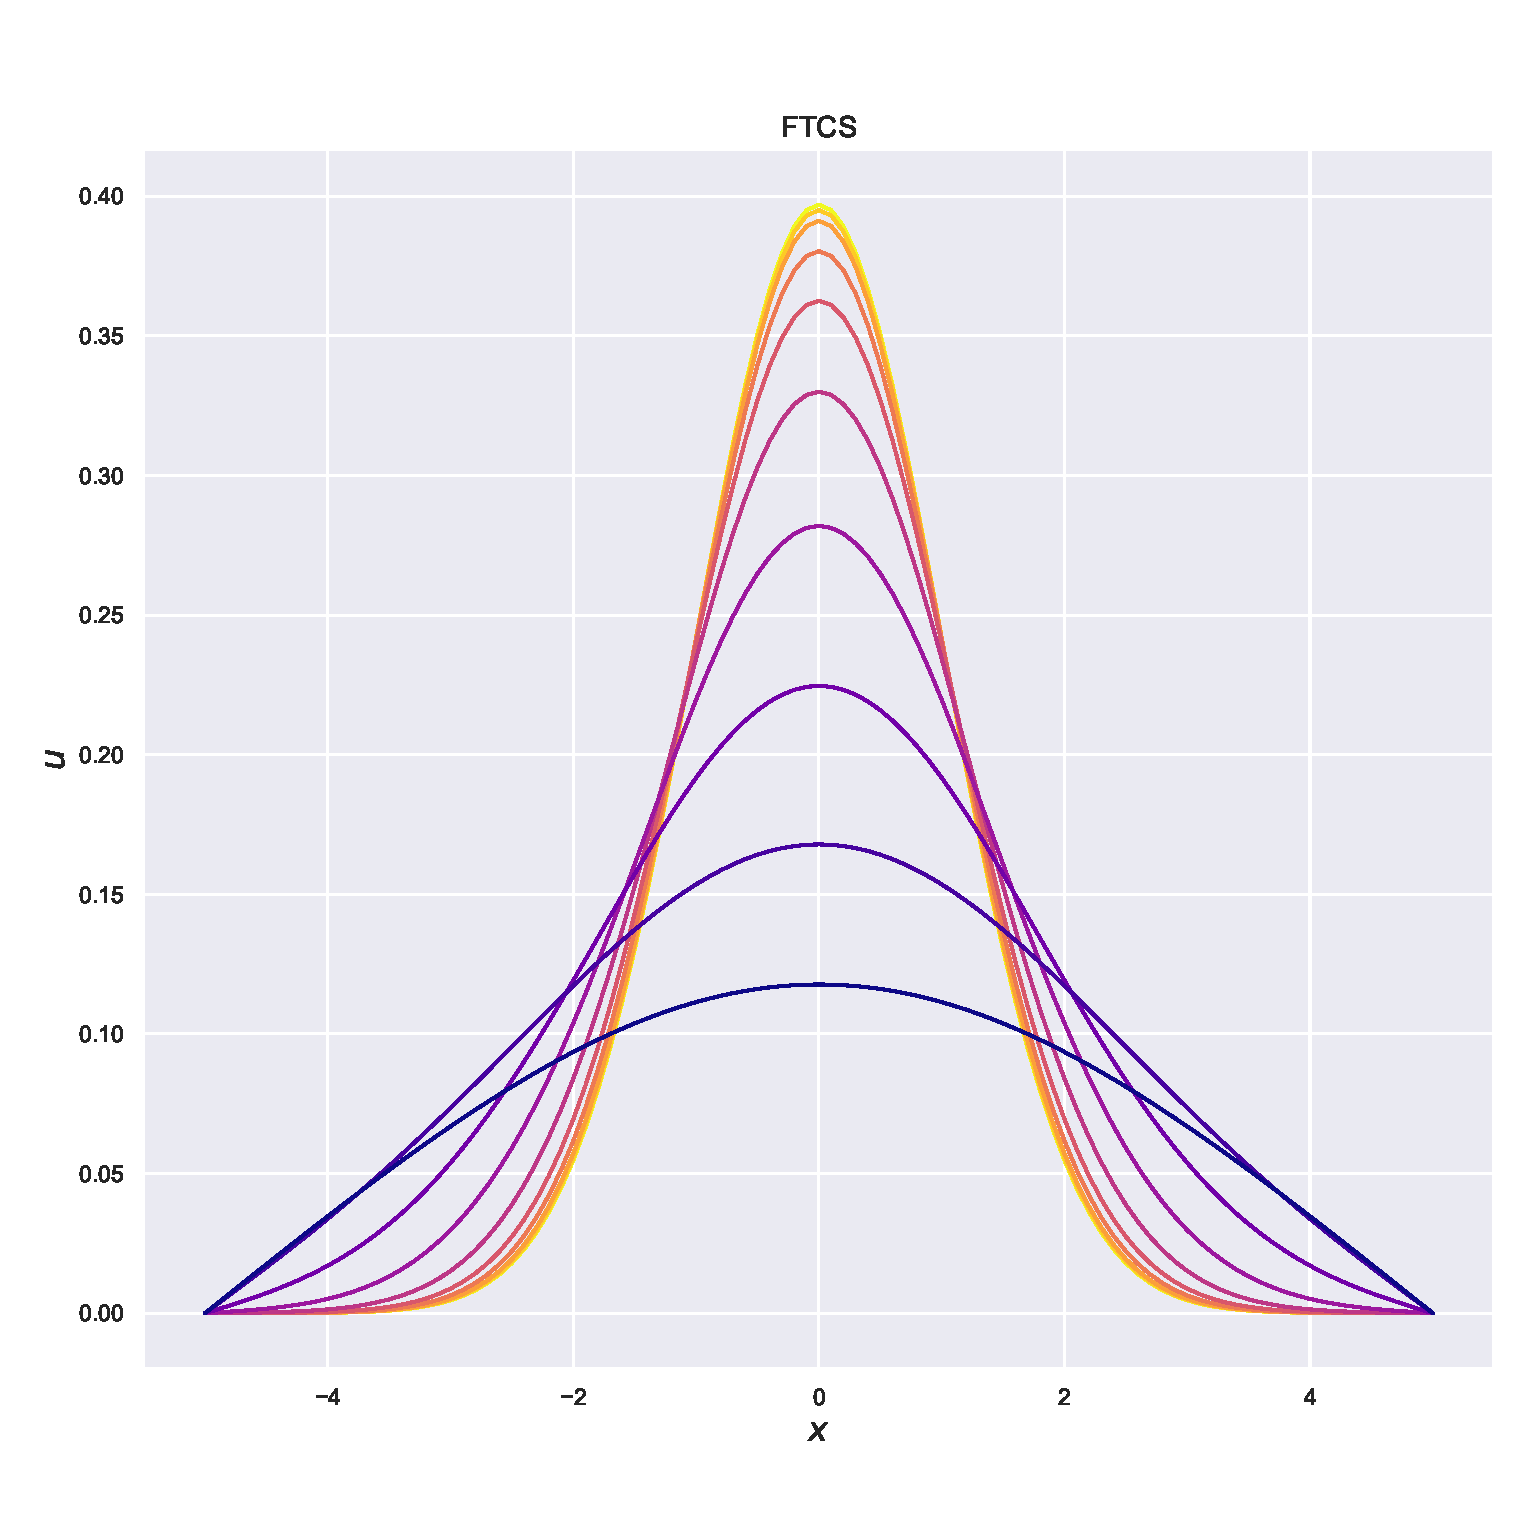
\includegraphics[width=\textwidth]{Figures/stableFTCSheat.eps}
        \subcaption{\(\Delta t = 0.005\)}
    \end{minipage} %
    \begin{minipage}[b]{0.49\textwidth}
        \centering
        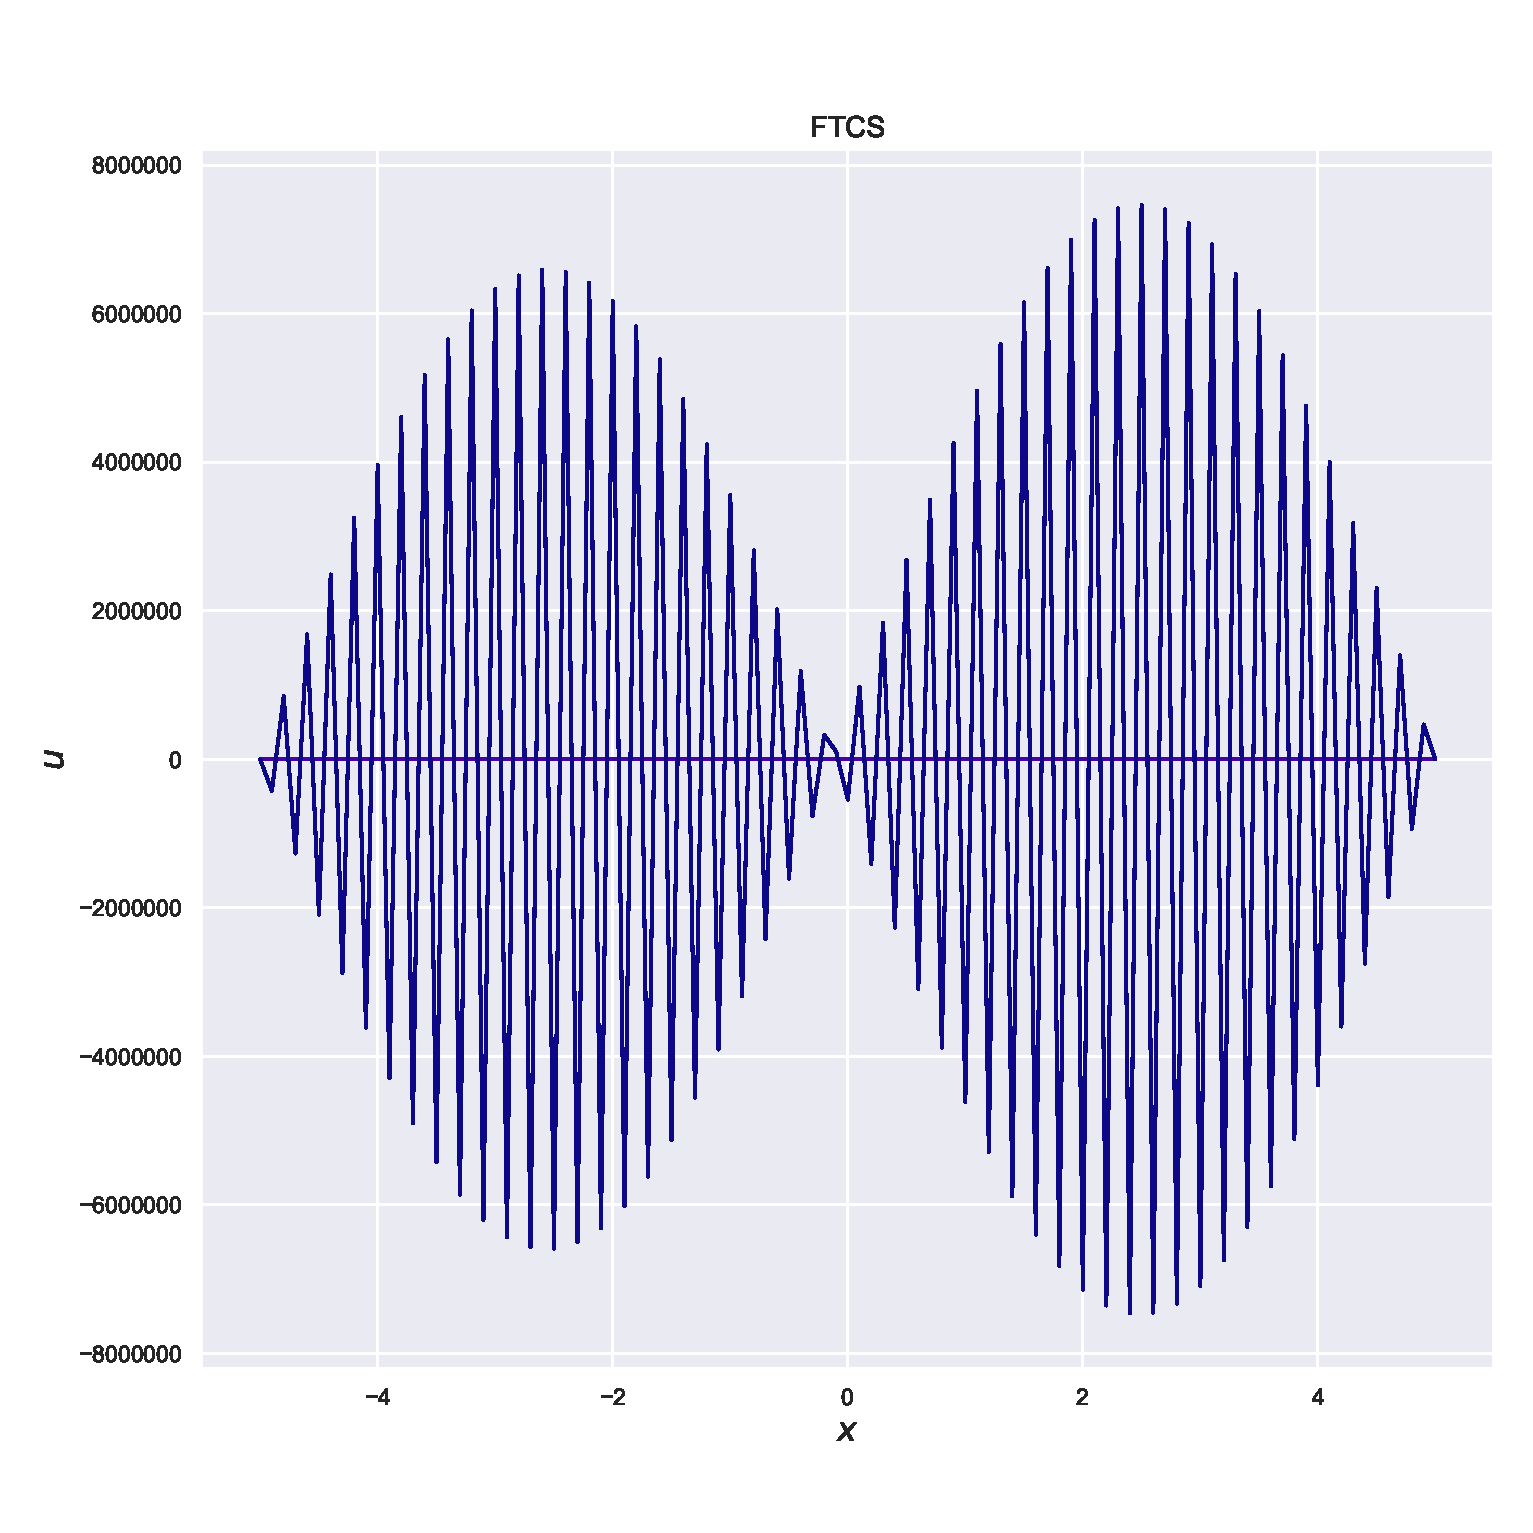
\includegraphics[width=\textwidth]{Figures/unstableFTCSheat.eps}
        \subcaption{\(\Delta t = 0.0051\)}
    \end{minipage} %
    \caption[Instability in the FTCS scheme]{Using the \texttt{FTCS} scheme to solve the heat equation \eqref{eq:heat} on \( \lbrack -5,5\rbrack \times\lbrack -1,1\rbrack\) with \(\sigma =1, \Delta x = 0.1\) with a Gaussian initial profile. When the stability condition is violated, $\lambda>1$ and the solution grows exponentially.} 
    \label{fig:FTCSunstable}
\end{figure}

A numerical scheme is consistent if the local truncation error tends to zeros as \(\Dx, \Dt \to 0\). The FTCS scheme is consistent of order one in time and two in space and stable so long as \(\mu \leq \frac{1}{2}\).  A scheme is convergent if for any fixed point  \((x^*,t^*) \in [-L,L] \times [0,T]\), \[x_j \to x^*, t_n \to t^* \implies U^n_j \to u(x^*,t^*).\]
The explicit scheme is convergent when it is stable. The stability condition is a great drawback of the FTCS method. In the next section we look to new methods to remove any restrictions on the mesh spacing, whilst maintaining (or improving) the truncation error.

\subsubsection*{Backward Time Centred Space}
If instead of looking at the forward time difference we look at the backward time difference, the scheme becomes stable. This is surprising, very little appears to change but the scheme is fundamentally different. This method is implicit, meaning that its solution requires a more complex calculation at every time step. However, the lack of restriction on the size of the timestep means fewer steps (and therefore fewer calculations) need to be performed. The backward time centred space (BTCS) scheme for \eqref{eq:heat} is
\begin{align}
\frac{U^{n+1}_j- U^n_j}{\Dt} &= \sigma \frac{U^{n+1}_{j+1} - 2U^{n+1}_{j} + U^{n+1}_{j-1}}{(\Dx)^2}.
%\label{eqBTCSheat}
\end{align}
The only difference here is the right hand side is calculated at the $n+1^{\text{th}}$ time step whereas in the FTCS algorithm it is taken at $n$. This scheme cannot be written explicitly in terms of known values, that is, the $n^{\text{th}}$ time step. Instead, we move all unknowns to the left hand side to give
\[
-\mu U^{n+1}_{j-1} + (1+2\mu)U^{n+1}_j - \mu U^{n+1}_{j+1} = U^n_j
\]
where, as before, $\mu=\frac{\Dt}{(\Dx)^2}$. This leads to a set of $J-1$ simultaneous equations. As the system is tridiagonal, the Thomas algorithm can be used to efficiently solve the system. See Appendix \ref{app:thomas} for a description.

The stability and consistency of the BTCS scheme can be found using the same techniques as was used for the explicit FTCS scheme. Assuming once again that the approximate solution as a Fourier mode, one obtains
\[\lambda = \frac{1}{1+4\mu \sin^2(\frac{1}{2}k\Dx)}.\]
This is less than one for any positive $\mu$, and so the BTCS method is unconditionally stable. The local truncation error of the scheme is the same as that of the FTCS method, namely the BTCS scheme is first order in time and second order in space. We now have a method with the same accuracy as the explicit scheme, but with no restriction on mesh size. The final method introduced will maintain this lack of constraint whilst increasing the accuracy, with little extra effort.
\begin{figure}
    \centering
    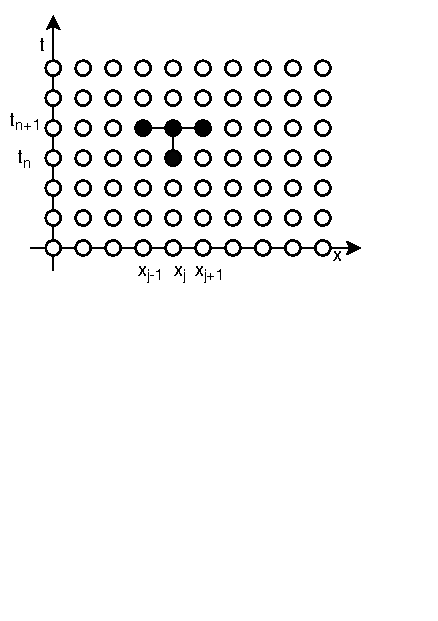
\includegraphics[width=0.5\linewidth, trim={0 5cm 0 0}, clip]{Figures/BTCS}
    \caption[BTCS stencil]{The points used in the implicit BTCS scheme}
    \label{fig:BTCSmesh}
\end{figure}

\subsubsection*{Theta Method}
So far we have considered two methods, each using a set of three points to update. Given that we know how to solve implicit and explicit methods is there an optimal hybrid between the two? The theta method aims to find this optimum by taking a weighted average of the FTCS and BTCS schemes. Applied to our toy problem \eqref{eq:heat}, the scheme is
\[
\frac{U^{n+1}_{j}-U^{n}_{j}}{\Dt} = \sigma\left(\theta \frac{U^{n+1}_{j+1}-2U^{n+1}_{j}+U^{n+1}_{j-1}}{(\Dx)^2}+(1-\theta)\frac{U^{n}_{j+1}-2U^{n}_{j}+U^{n}_{j-1}}{(\Dx)^2}\right),
\]
where $0\leq \theta 1$ is a weighting parameter. For $\theta = 0$, the FTCS scheme is recovered, and likewise when $\theta = 1$ the scheme is just the BTCS method. The aim of this section is to find an optimum weight for $\theta$, if one exists. Optimum here means the value that decreases the truncation error the most, whilst maintaining the unconditional stability of the BTCS method. Rearranging as a tridiagonal system gives
\[
-\theta\mu U^{n+1}_{j-1} + (1+2\theta\mu)U^{n+1}_j - \theta\mu U^{n+1}_{j+1} = U^n_j + (1-\theta)\mu \left[U^n_{j+1} - 2U^n_{j} + U^n_{j-1} \right]. 
\]

Using the stability analysis from the FTCS scheme, one obtains
\[ \lambda = \frac{1-4(1-\theta)\mu\sin^2(\frac{1}{2}k\Dx)}{1+4\theta\mu\sin^2(\frac{1}{2}k\Dx)}.\]
Note again that if $\theta = 1$, $\lambda$ is as it was for the BTCS scheme, and if $\theta = 0$, the value for the FTCS method is recovered. This is always less than one and is greater than minus one if
\[\mu(1-2\theta) \leq \frac{1}{2}.\]
Hence any choice of $\theta \geq \frac{1}{2}$ is sufficient for unconditional stability. This makes intuitive sense: the BTCS method is unconditionally stable, so any weighting preferring this scheme is also stable. If $\theta > \frac{1}{2}$, the mesh spacing can be adjusted to retain stability, as in the FTCS method. 
\begin{figure}
    \centering
    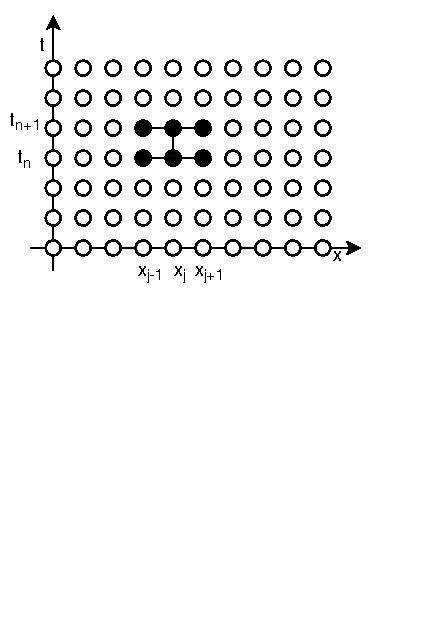
\includegraphics[width=0.5\linewidth, trim={0 5cm 0 0}, clip]{Figures/CN}
    \caption[Theta Method Stencil]{Points used in the Theta method}
    \label{fig:CNmesh}
\end{figure}
Thus far there is no reason to prefer the theta method over the simpler BTCS scheme. However, let's consider the truncation error of the scheme using similar analysis as above, expanding this time around the midpoint of the mesh, $(x_j, t_{n+\frac{1}{2}})$.
    \[\begin{split}R^{n+\frac{1}{2}}_j = \lbrack \partial_t u - \partial_{xx}u\rbrack &+ \left[\left(\frac{1}{2} - \theta\right)\Dt \partial_{xxt}u - \frac{1}{12}(\Dx)^2\partial^4_{x} u\right]\\&+\left[\frac{1}{24}(\Dt)^2\partial^3_{t}u - \frac{1}{8}(\Dt)^2u_{xxtt}\right]\\
    &+\left[\frac{1}{12}\left(\frac{1}{2}-\theta\right)\Dt (\Dx)^2\partial_{xxxxt}u - \frac{2}{6!}(\Dx)^4\partial^6_xu\right]
    \end{split} \]
So for arbitrary choice of $\theta$, the scheme remains first order in time and second order in space. However, if $\theta=\frac{1}{2}$, the first order in time term is zero, and the scheme is second order in both time and space. The optimal value of $\theta$ is the even weighting of the FTCS and BTCS scheme. This method is known as the Crank-Nicolson (CN) method, and is the first choice when using finite difference methods -- it is simple, quick and accurate to second order. Table \ref{tab:FDmethods} summarises the results of this section. The supplementary notebook contains all three solvers for the heat equation \eqref{eq:heat}. For the model, a Crank-Nicolson scheme will be used.
\begin{table}
    \centering
    \begin{tabular}{|c|c|c|c|}
        \hline
        & & & \\[-0.5em] 
        Method & FTCS ($\theta=0$) & BTCS ($\theta=1$) & Crank-Nicolson ($\theta=\frac{1}{2}$) \\[0.3em] 
        \hline 
        & & & \\[-0.5em] 
        LTE & $\mathcal{O}(\Dt), \mathcal{O}(\Dx^2)$ & $\mathcal{O}(\Dt), \mathcal{O}(\Dx^2)$ & $\mathcal{O}(\Dt^2), \mathcal{O}(\Dx^2)$ \\[0.3em]  
        \hline
        & & & \\[-0.5em]  
        Stablity Condition & $\mu\leq \frac{1}{2}$ & None & None \\[0.3em]  
        \hline 
        & & & \\[-0.5em] 
        Explicit/Implicit & Explicit & Implicit & Implicit \\[0.3em]  
        \hline 
    \end{tabular}
\caption{Finite difference methods for diffusion equations}
\label{tab:FDmethods}
\end{table}

\begin{figure}
    \centering
    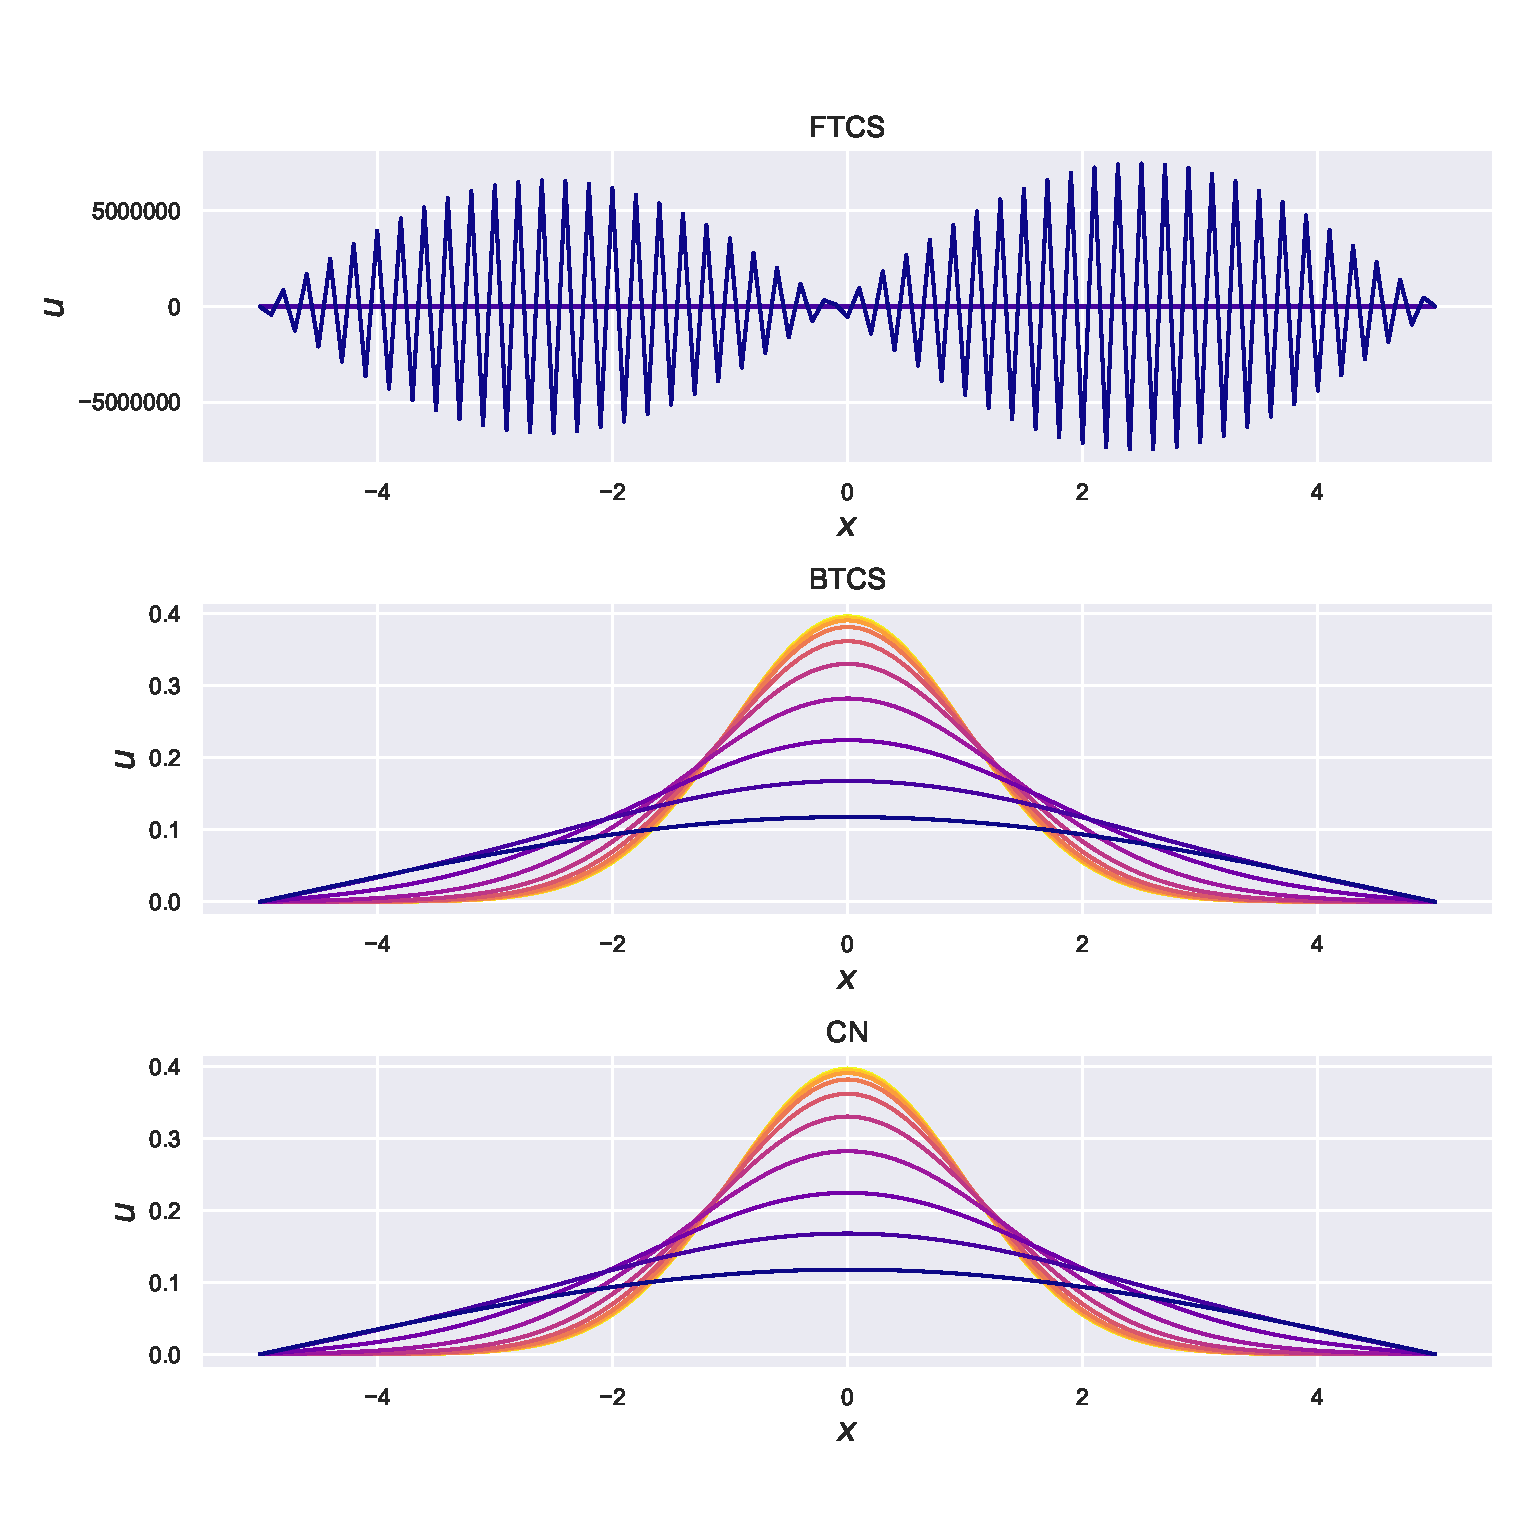
\includegraphics[width=0.7\linewidth]{Figures/FTCSandCN}
    \caption[Comparison of FTCS, BTCS, CN solvers]{Solving the heat equation as in Figure \ref{fig:FTCSunstable} using FTCS, BTCS and CN solvers respectively. The implicit solvers remain stable regardless of step size, and return an accurate solution.}
    \label{fig:ftcsandcn}
\end{figure}
\subsection{Advection Equations}
Our prototypical example in this case will be the one-way wave equation,
\begin{equation}\label{eq:wave}\begin{cases}
\partial_t u(t,x) + a(x)\partial_x u(t,x)=0,\\
u(0,x) = u_0(x),  &t\in\R^+, x\in\R.
\end{cases}\end{equation}
Advection equations are, in general, much more difficult to solve numerically than the diffusion equation. In this section we will consider $a$ constant to illustrate the methods. When solving an advection equation numerically, any scheme must satisfy the CFL condition. To motivate the choice of scheme, we first introduce this condition.

The exact solution to an advection equation can be found by using the method of characteristics. Characteristics are lines on which the PDE \eqref{eq:wave} reduces to an ODE. Let 
\[\od{x}{t} = a(x,t).\]
Then using the chain rule,
\[
\od{u}{t} = \partial_t u +\od{x}{t}\partial_x u = 0,
\]
as $u$ solves the PDE. Thus on a characteristic, the solution is constant. For the case when $a$ is constant, the characteristics are the straight lines $x-at = const.$ and the solution is \[ u(x,t) = u_0(x-at).\] The initial profile is simply transformed at a speed $a$. The solution at a point $(x_j,t_n)$ is then obtained by finding the characteristic through this point and following it backwards in time to $t=0$. If a discretisation is applied to equation \eqref{eq:wave}, we obtain the explicit scheme
\[\frac{U^{n+1}_j-U^n_j}{\Dt} =-a \frac{U^n_{j+1}-U^n_j}{\Dx}.\] 
As in the FTCS method, to find the value of the solution at the next time point we evaluate
\[U^{n+1}_j = U^n_j - c(U_{j+1}-U_j), \]
where $c=\frac{a\Dt}{\Dx}$. Figure \ref{fig:CFL} shows the dependence of the current point on all previous points. Each point depends on two points from the previous time level, propagating all the way back to the initial line. This set of points, here a triangle, is the domain of dependence of the scheme. The CFL condition states that for a scheme to converge the characteristic curve passing through a point must stay within the domain of dependence for that point. In Figure \ref{fig:CFL}, two example characteristics are plotted for $a>0 (PQ)$ and for $a<0 (PR)$. The explicit scheme outlined above is then only convergent for negative values of $a$, otherwise the characteristic lies outside of the domain of dependence. Intuitively, a scheme cannot be accurate if it cannot `see' the wave arriving. If the wave is moving too fast, the CFL condition may be violated as the characteristic becomes much shallower and again lies outside the domain of dependence of the numerical scheme. This can be counteracted by reducing the timestep, effectively widening the base of the domain of dependence until it includes the characteristic. For this scheme this requires 
\[c =\frac{a\Dt}{\Dx} < 1.\]
\begin{figure}
    \centering
    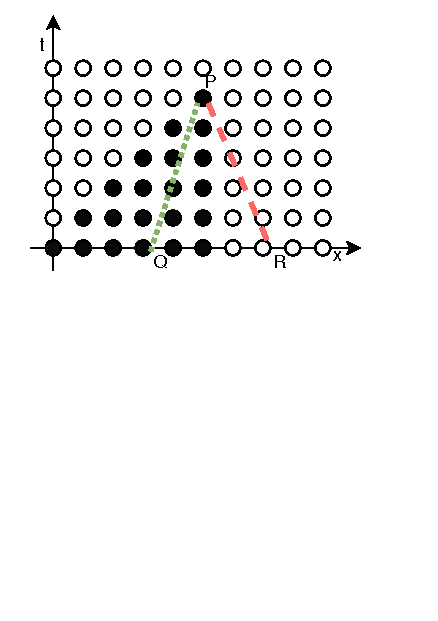
\includegraphics[width=0.7\linewidth, trim={0 5cm 0 0}, clip]{Figures/CFL}
    \caption[CFL Condition]{}
    \label{fig:CFL}
\end{figure}
This condition ensures the solution does not travel further in one time step than one spacestep, thereby remaining in the domain of dependence. This condition is dependent on the geometry of the domain of dependence. The CFL condition is necessary but not sufficient for stability, as the following scheme shows. One way to satisfy the condition would be to make the triangle isosceles instead of right-angled. This can be achieved by taking a central difference in space:
\[
    \frac{U^{n+1}_j-U^n_j}{\Dt} =-a \frac{U^n_{j+1}-U^n_{j-1}}{\Dx}
\]
The CFL condition here requires $|a|\frac{\Dt}{\Dx} < 1$. By applying the stability analysis used for the FTCS method, one obtains $\lambda = 1-c i \sin(k\Dx)$. This is always greater than one, and the scheme is thus unconditionally unstable, despite satisfying the CFL condition. The upwind scheme is the simplest stable method for advection equations. It switches the direction of the difference based on the direction of the wave, thereby always `facing into the wave' (upwind).
\[
U^{n+1}_{j} = \begin{cases} U^{n}_{j}-c(U^{n}_{j+1}-U^{n}_{j}) & \text{ if } a<0\\[0.5em]
U^{n}_{j}-c(U^{n}_{j}-U^{n}_{j-1}) & \text{ if } a>0\\
\end{cases}
\]
Satisfying the CFL condition here requires $|a|\frac{\Dt}{\Dx} < 1$, and in fact stability analysis shows this is also sufficient for stability. Furthermore, the local truncation error can be calculated. Here we set $a>0$.
\begin{align*}
    R^n_j &= \frac{u^{n+1}_j-u^n_j}{\Dt}  + a \frac{u^n_{j}-u^n_{j-1}}{\Dx}\\
    &=\frac{1}{2}(\Dt \partial^2_t u - a\Dx \partial^2_x u)+\dots
\end{align*}
So the upwind scheme is first order in both time and space. Higher order schemes are available for advection equations, however this will suffice for a first approximation to the model. There are problems, however, with artificial dissipation in this scheme, as Figure \ref{fig:advection} shows. For a heuristic insight, we can consider the modified equation. By a Taylor expansion in the upwind scheme, we obtain
\[\frac{u^n_j - u^n_{j-1}}{\Dx} = \partial_x u^n_j + \frac{1}{2}\Dx\partial^2_{x}u^n_j + \mathcal{O}(\Dx^2). \]
This shows that the numerical solution will be more closely approximating an advection-diffusion equation:
\[\tilde{u}_t + a\tilde{u}_x = \frac{1}{2}a\Dx\partial^2_x \tilde{u}.\]
The modified equation shows the source of the dissipative effects seen in the scheme.
\begin{figure}
    \centering
    \begin{minipage}[b]{0.49\textwidth}
        \centering
        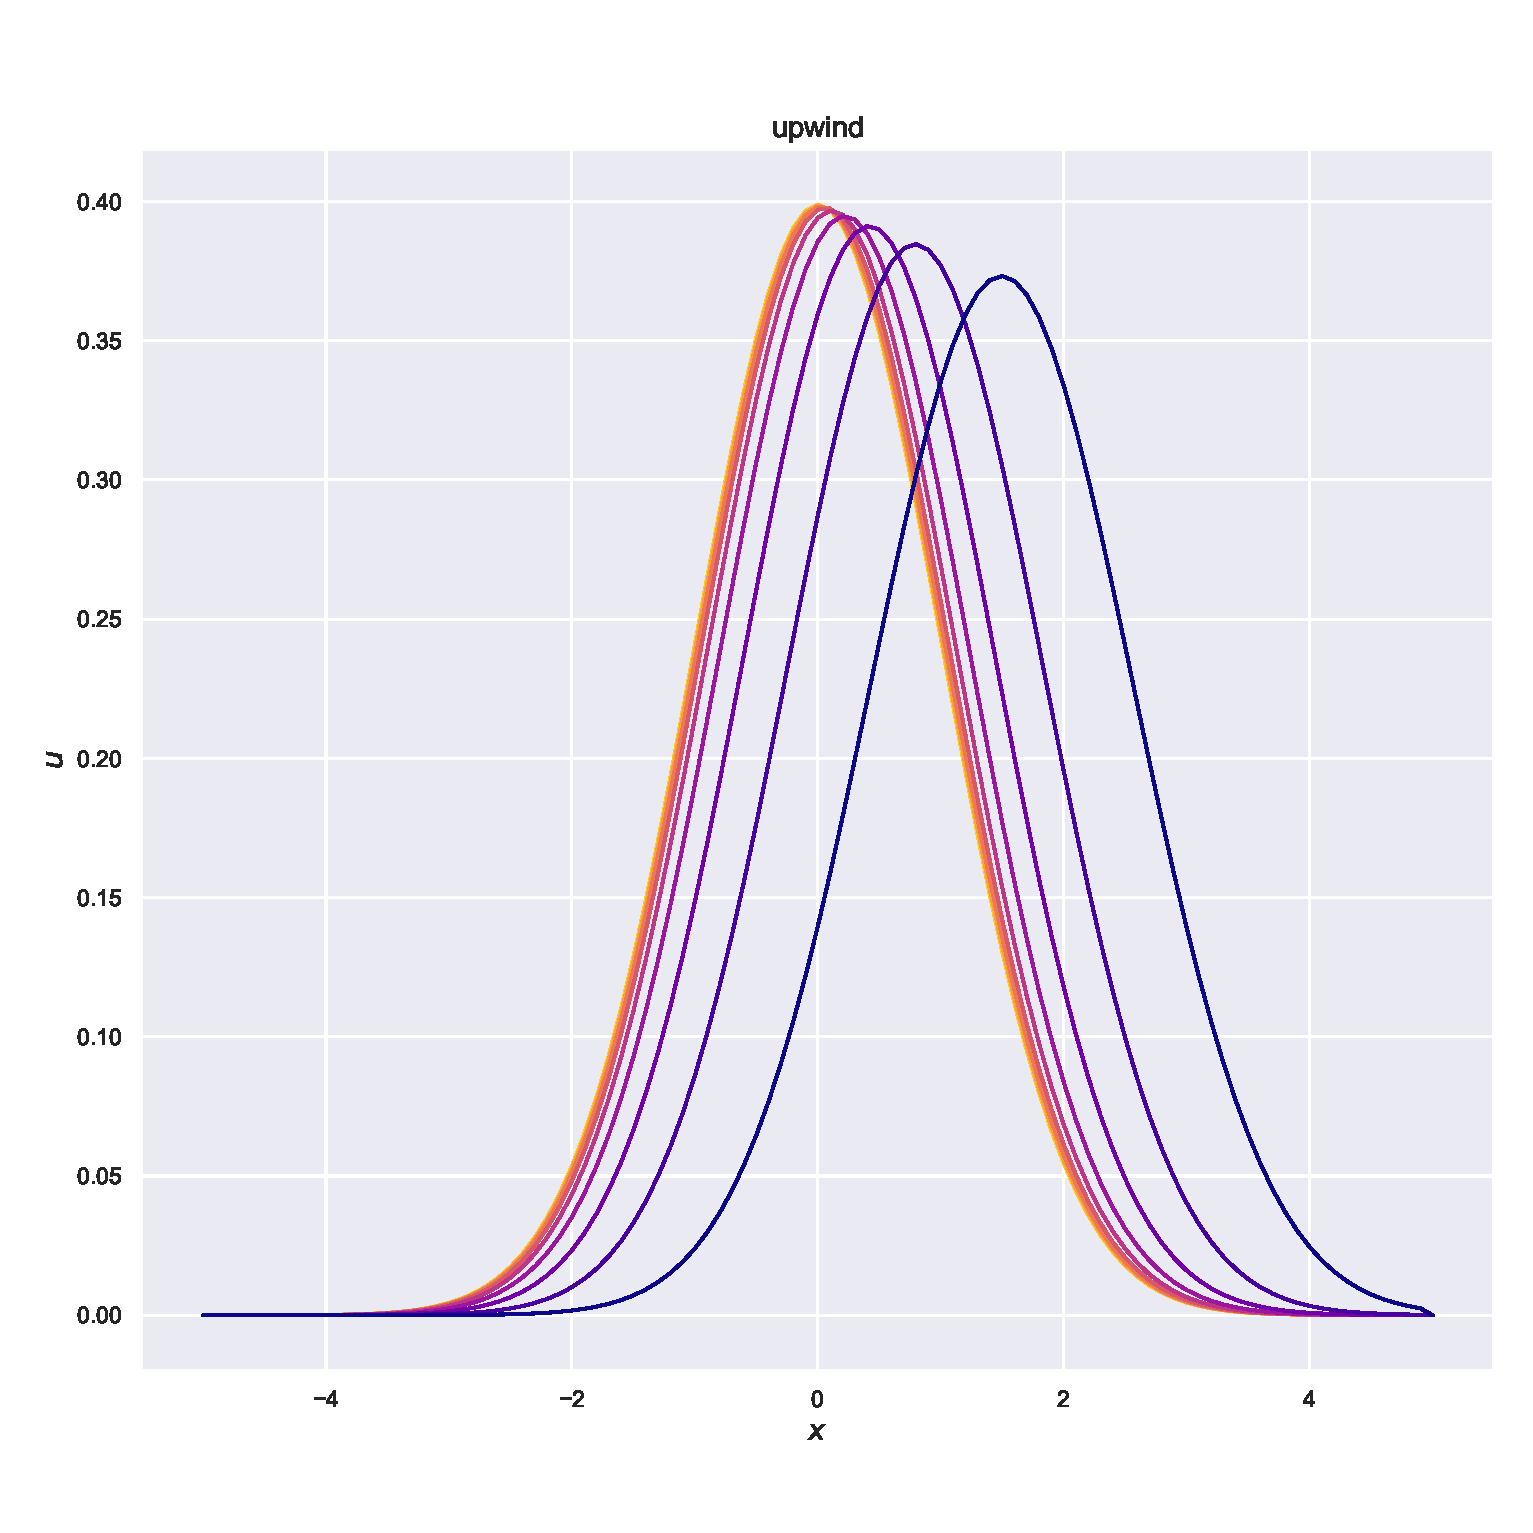
\includegraphics[width=\textwidth]{Figures/advgaussian.eps}
        \subcaption{$U_0 \sim \mathcal{N}(0,1)$}
    \end{minipage} %
    \begin{minipage}[b]{0.49\textwidth}
        \centering
        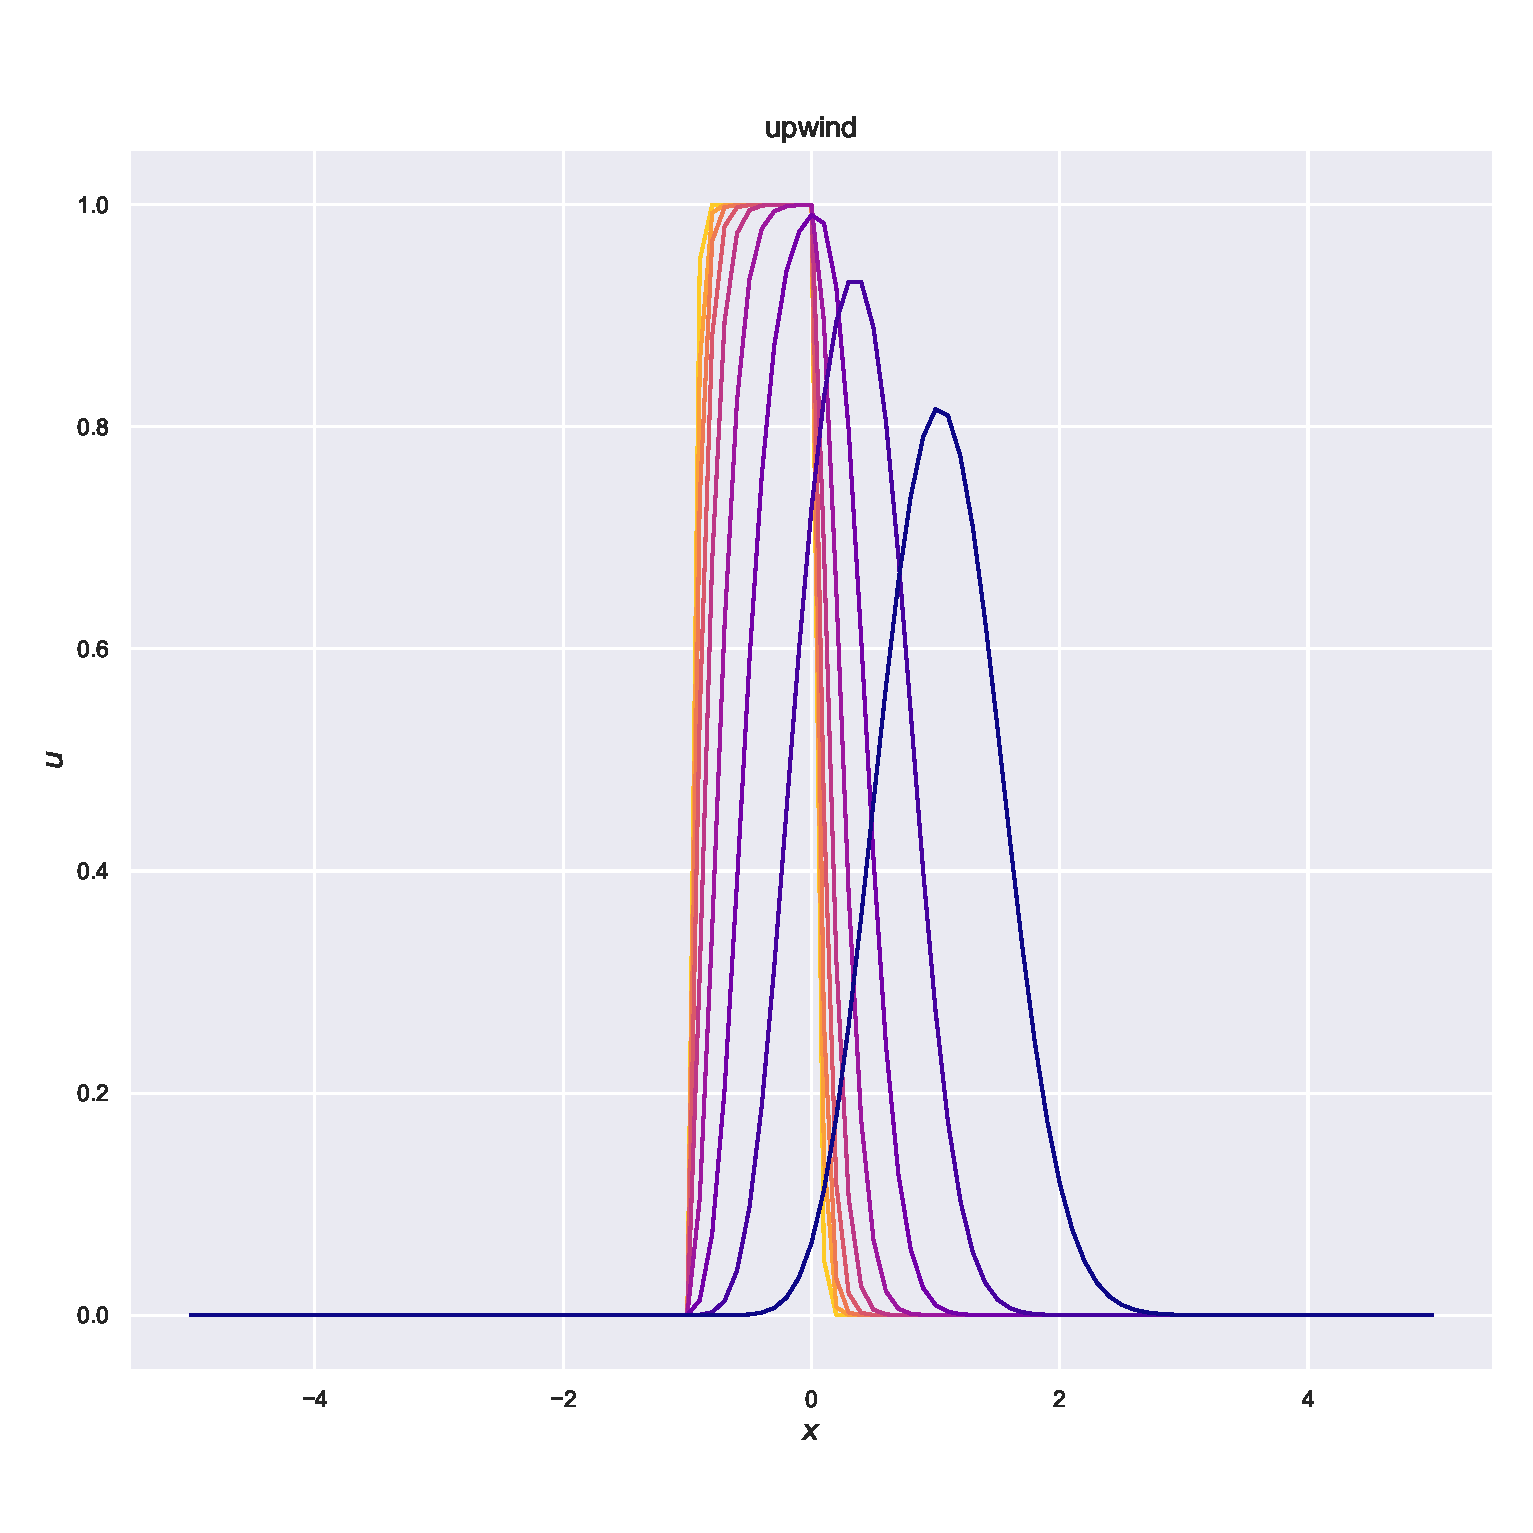
\includegraphics[width=\textwidth]{Figures/advindicator.eps}
        \subcaption{$U_0(x) = \mathbbm{1}_{\lbrack-1,0\rbrack}(x)$}
    \end{minipage} %
    \caption{Solving equation \eqref{eq:wave} with the upwind scheme. Even with very smooth initial data, dissipative effects can be severe.} 
    \label{fig:advection}
\end{figure}
\subsubsection*{Finite Volume Schemes}
One aspect of the advection equation \eqref{eq:wave} the schemes thus far have not yet exploited is its conservation of mass. Finite volume methods ensure mass is conserved in the scheme, something not yet considered that can be a source of error. Finite volume schemes can be applied to any conservation (or continuity) equation. A conservative equation is one that can be written in the form
\[\partial_t u + \partial_x(a(x) u).\]
On the same mesh as previously, auxiliary points are introduced between points in space, namely $x_{j+\frac{1}{2}}$ for $0\geq j \leq J-1$. Within any interval (or volume), $\Omega_j = \left[x_{j-\frac{1}{2}},x_{j+\frac{1}{2}}\right]$, we can calculate the average density.
\[\bar{u}(x_j) = \frac{1}{\Dx}\int_{\Omega_j} u(x) \dif x = u(x_j) + \frac{(\Dx)^2}{24}\partial^2_x u(x_j) +\dots \]

Furthermore, the change in the average density within the cell is equal to difference of the mass lost through the boundary of the volume, that is,
\[
\Dx\od{\bar{u}(x_j)}{t} = a(x_{j-\frac{1}{2}})u(x_{j-\frac{1}{2}}) - a(x_{j-\frac{1}{2}})u(x_{j-\frac{1}{2}}), 
\]
This is also known as the flux across the boundary. A finite volume scheme balances fluxes across the domain, thereby maintaining total mass. Doing so leads to the first-order upwind scheme in flux form,
\[
\frac{U^{n+1}_j - U^n_j}{\Dt} = \frac{-1}{\Dx}\left[ a(x_{j+\frac{1}{2}})U^n_{j+\frac{1}{2}} - a(x_{j-\frac{1}{2}})U^n_{j-\frac{1}{2}}\right].  
\]
The value of $a$ at the midpoint is chosen to be the average of its value at the cell centres, that is $a(x_{j+\frac{1}{2}}) = \frac{1}{2}\left(a(x_j)+a(x_{j+1})\right)$. The scheme as written will be unstable if $a(x)<0$, for the same reason as in the previous section. The spatial bias needs to be changed depending on the direction of the wave. 
\[
a(x_{j+\frac{1}{2}})U^n_{j+\frac{1}{2}} = a^+(x_{j+\frac{1}{2}})U^n_{j} + a^-(x_{j+\frac{1}{2}})U^n_{j+1},
\]
where $a^+ = \max(a,0), a^- = \min(a,0)$.  This scheme is still order 1, however it provides the ideal setting for developing higher order schemes.
 
    \section{Applying the Numerical Scheme}\label{sec:application}
        We now have enough methods to begin approximating both the particle system and the kinetic model. As in previous sections, we first focus on the particle system, before involving the continuum approach. 
\subsection{Space-Homogeneous Particle Model}\label{sec:homparticles}
Recall the homogeneous particle model \eqref{eq:homparticle},
\begin{equation}\tag{\ref{eq:homparticle}}
\dif v^{i,N}_t = G\left(\frac{1}{N}\sum_{j=1}^n v^{j,N}_t\right)\dif t-v^{i,N}_t \dif t + \sqrt{2\sigma} \dif W^i_t.
\end{equation}
Simulating this system is analagous to solving the Ornstein-Uhlenbeck process of Section \ref{sec:particlemethods}. The interaction term is easily calculable using NumPy's \texttt{mean()} function as it is simply the average velocity of all the particles at each time step. The Euler-Maruyama scheme for this system is
\[ v^{i,N}_{n+1} = v^{i,N}_n - v^{i,N}_n\Dt + G\left(\frac{1}{N}\sum_{j=1}^N v^{j,N}_n\right)\Dt+ \sqrt{2\sigma\Dt} Z^i_n. \]
As the system contains interactions, simulating one particle for a long time is no longer sufficient. Multiple particles must be simulated simultaneously. Figure \ref{fig:homparticlemoments} shows how the particle system behaves for a uniform initial distribution with negative mean. The mean velocity is herded towards -1, as predicted in the analysis. The variance behaves similarly, moving towards an average value of 1. Here the mean and variance of velocity is taken at each time step. If instead these statistics were taken across all time up to the point, by setting \texttt{timeavg = True}, the convergence is more clear.
\begin{figure}
    \centering
    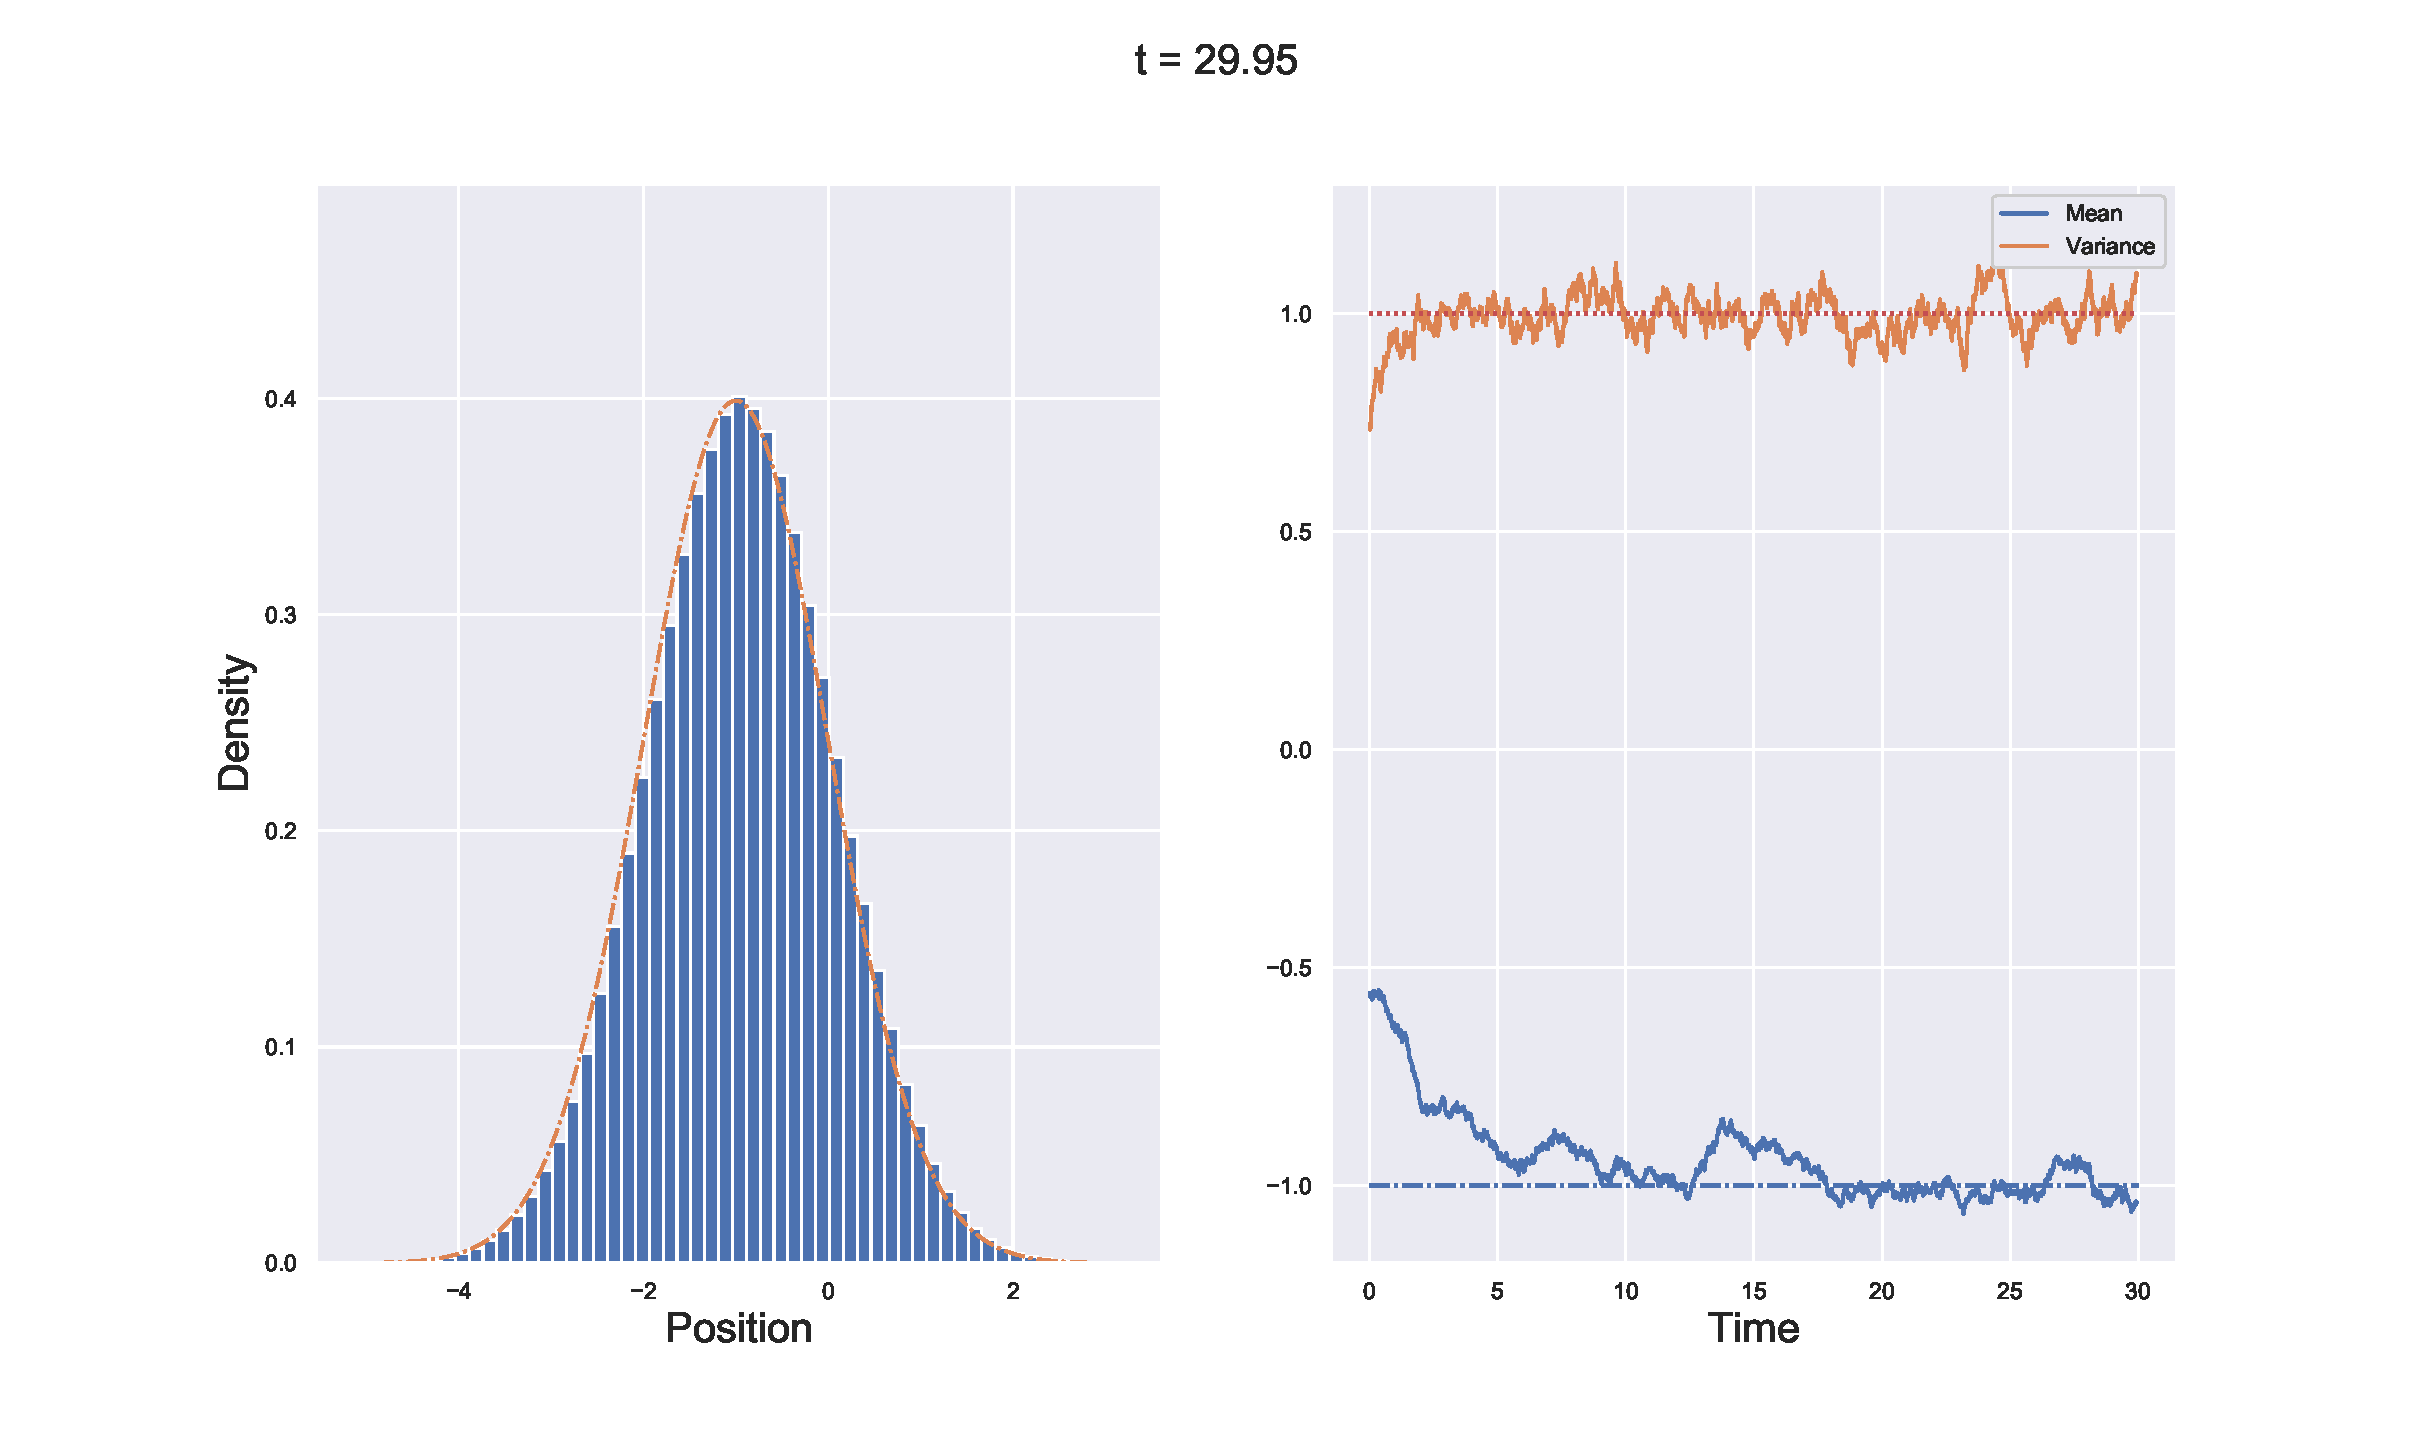
\includegraphics[width=\linewidth]{Figures/homparticles}
    \caption[Homogeneous Particle System]{Histogram of velocities of 1000 particles after 30s with $\sigma = 1$ against the analytic stationary distribution. A time step of $\Dt = 0.01$ was used and the initial data was uniform on $[-2,1]$. The right-hand plot shows the mean and variance moving towards the predicted values and oscillating about them.}
    \label{fig:homparticlemoments}
\end{figure}
We can also plot an animation of the movement of the density of particles over time. Recall from Section \ref{sec:dynamics} that the empirical distribution of the particle system only approximates the true distribution as the number of particles tends to infinity. For any finite number of particles there is only one stationary distribution. When simulating the system, if the number of particles is high enough the probability that enough particles jump across the barrier is very small, and will only be seen if the simulation is ran for an extremely long time. Nevertheless, if the number of particles is low enough, these switches happen often enough to observe, as Figure \ref{fig:switch} shows. This something to be aware of when comparing the kinetic model with the particle model -- a low number of particles produces a better approximation to the invariant distribution of the particle system, but a worse approximation of the kinetic model solution.

\begin{figure}
    \centering
    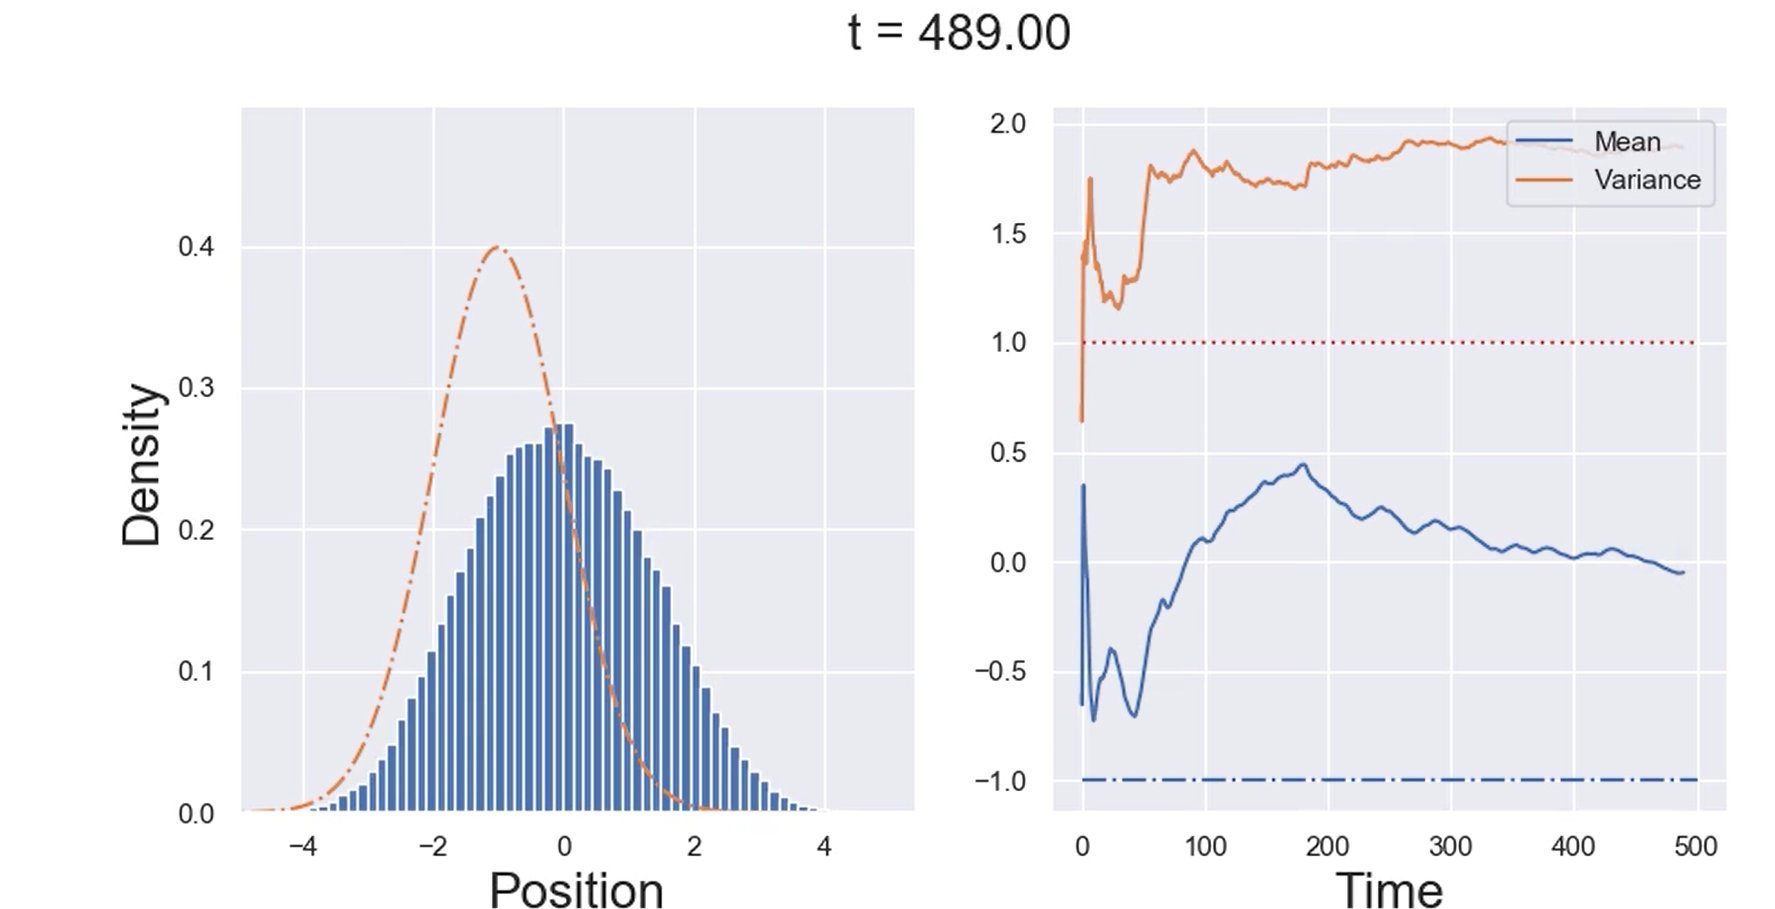
\includegraphics[width=\linewidth]{Figures/switch}
    \caption[Mean Zero Invariant Measure for the Particle System]{When simulated for a long time with a low number of particles (here there are 6, and $T=500$) the particles do not behave as the kinetic model predicts.}
    \label{fig:switch}
\end{figure}

+++List of things that can be done in code?+++

\subsection{Space-Homogeneous Kinetic Model}\label{sec:homkin}
 Consider the space-homogeneous evolution given by \eqref{eq:spacehomPDE}, that is
    \begin{equation}
    \partial_t f_t(v) = \partial_v vf_t(v) - \partial_v G(\langle w \rangle_{f_t})f_t(v) + \sigma \partial_{vv} f_t(v).\tag{\ref{eq:spacehomPDE}}
    \end{equation}
    Using the methods developed in Section \ref{sec:numericalmethods}, we are now able to approximate this system numerically. As when solving the heat equation, a zero boundary condition shall be enforced. This is valid as we know that the stationary distributions are Gaussian and centred at $-1,0,+1$. The boundary $L$ can then be chosen depending on the the diffusion so that almost no mass is contained beyond the boundary. For example if $\sigma = 1$, the mass contained beyond $L=5$ is of the order $10^{-5}$. 
    
    Simpson's rule will be used as a quick way to approximate the integral within the herding coefficient. To differentiate between the integral and its approximation, we write \(\langle w\rangle_{F^n}\). Below is the scheme when both the herding coefficient and the velocity are positive, using a finite difference scheme with a CN discretisation for the diffusive term and an upwind method for the damping and herding terms.
    \begin{equation*}
    \begin{split}
    \frac{F_j^{n+1} - F_j^n}{\Delta t} = 	-G(\langle w\rangle_{F^n})\left[ \frac{F^n_{j+1} - F^n_{j}}{\Delta v}\right] &+\left[ \frac{v_{j}F^n_{j} - v_{j-1}F^n_{j-1}}{\Delta v}\right]\\ &+ \frac{\sigma}{2}\left[ \frac{F^{n+1}_{j+1} - 2F^{n+1}_j + F^{n+1}_{j-1}}{(\Delta v)^2} + \frac{F^{n}_{j+1} - 2F^{n}_j + F^{n}_{j-1}}{(\Delta v)^2}\right] 	 
    \end{split}
    \end{equation*}
    This scheme will be first order in both time and space due to the use of the first-order upwinding. The stability will be restricted by the CFL condition, in particular, $\frac{|v_j-G(\langle w\rangle_{F^n})|\Dt}{\Dx} \leq 1$. A finite volume scheme has also been implemented. In this scheme the flux out of the right boundary is given by 
     \[ \max(0, v_{j+\frac{1}{2}}-G(\langle w\rangle_{F^n}))F^n_{j+1} + \min(0, v_{j+\frac{1}{2}}-G(\langle w\rangle_{F^n}))F^n_j + \frac{\sigma(F^n_{j+1} - F^n_j)}{\Dv}.
     \]
     This is a simple FTCS method applied to the diffusion term and a first order upwind on the advective term. The stability here is limited by the mesh spacing, however it illustrates the use of a finite volume method without incorporating an implicit solver. Figure +++ref+++ is a frame from an animation of the PDE solution approximated using the finite difference scheme compared with the particle system. The finite difference method appears to closely follow the behaviour of the particle system, so long as the number of particles is high enough. Figure \ref{fig:kinmodelmomvar} shows the first moment and the variance contrasted with the analytic solution of \eqref{eq:momode}. This clearly shows the almost immediate artificial dissipative effects of the upwind scheme in the finite volume case. The finite difference scheme appears to be better approximating the variance, however the spatial bias within this algorithm is not correct. Both schemes report no mass loss to 6 decimal places. This will be the case as long as the initial distribution does not have non-negligible mass at the boundary.
     
     The error in the approximate stationary distribution can be approximated by simply finding the difference between the analytic invariant measure and the approximate solution. Figure \ref{fig:homkinerror} shows exactly this for $\sigma = 1, \Dt = 0.001, T = 20, L=6, \Dv = 0.1$ and Gaussian initial data. The spatial bias in the finite difference method has introduced a bias in the error. No such bias exists for the upwinding in the finite volume solution, although the error is greater. This is very important for our aim in this project. If the initial data has mean zero, the scheme may always converge in the direction of the spatial bias, obscuring the true behaviour. 
     \begin{figure}
        \centering
        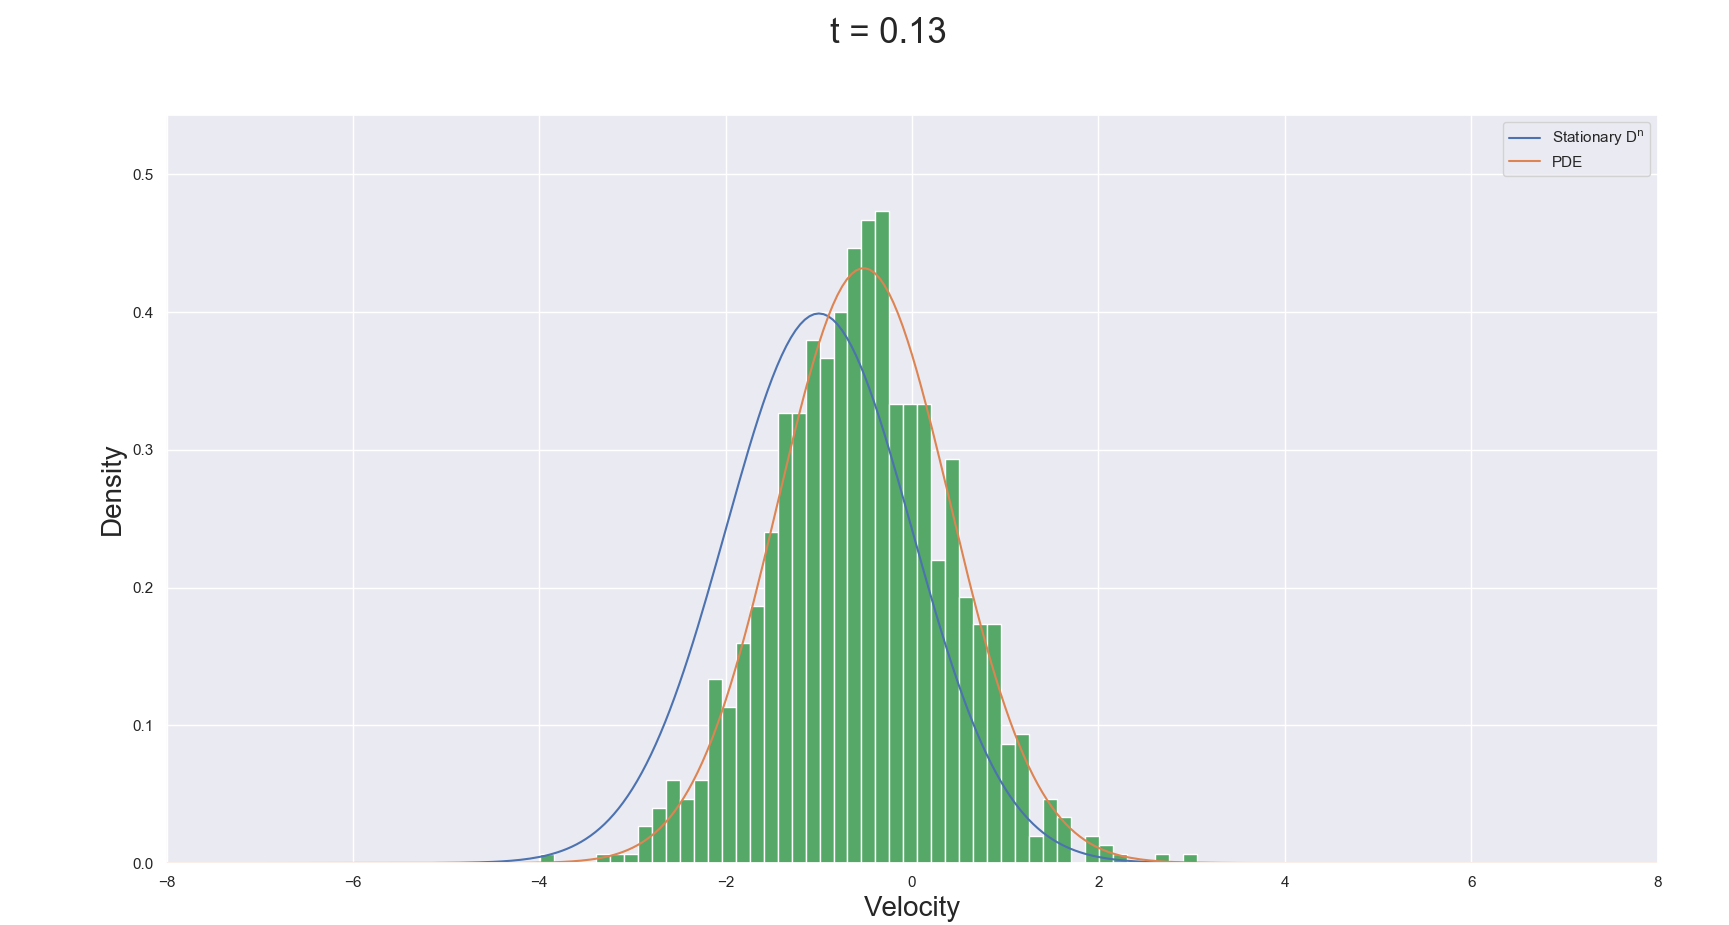
\includegraphics[width=\linewidth]{Figures/homPDEparticle}
        \caption[Comparing PDE to Particle Density]{Frame from animation of finite difference model against the particle model histogram.}
        \label{fig:homPDEparticle}
    \end{figure}
    \begin{figure}
        \centering
        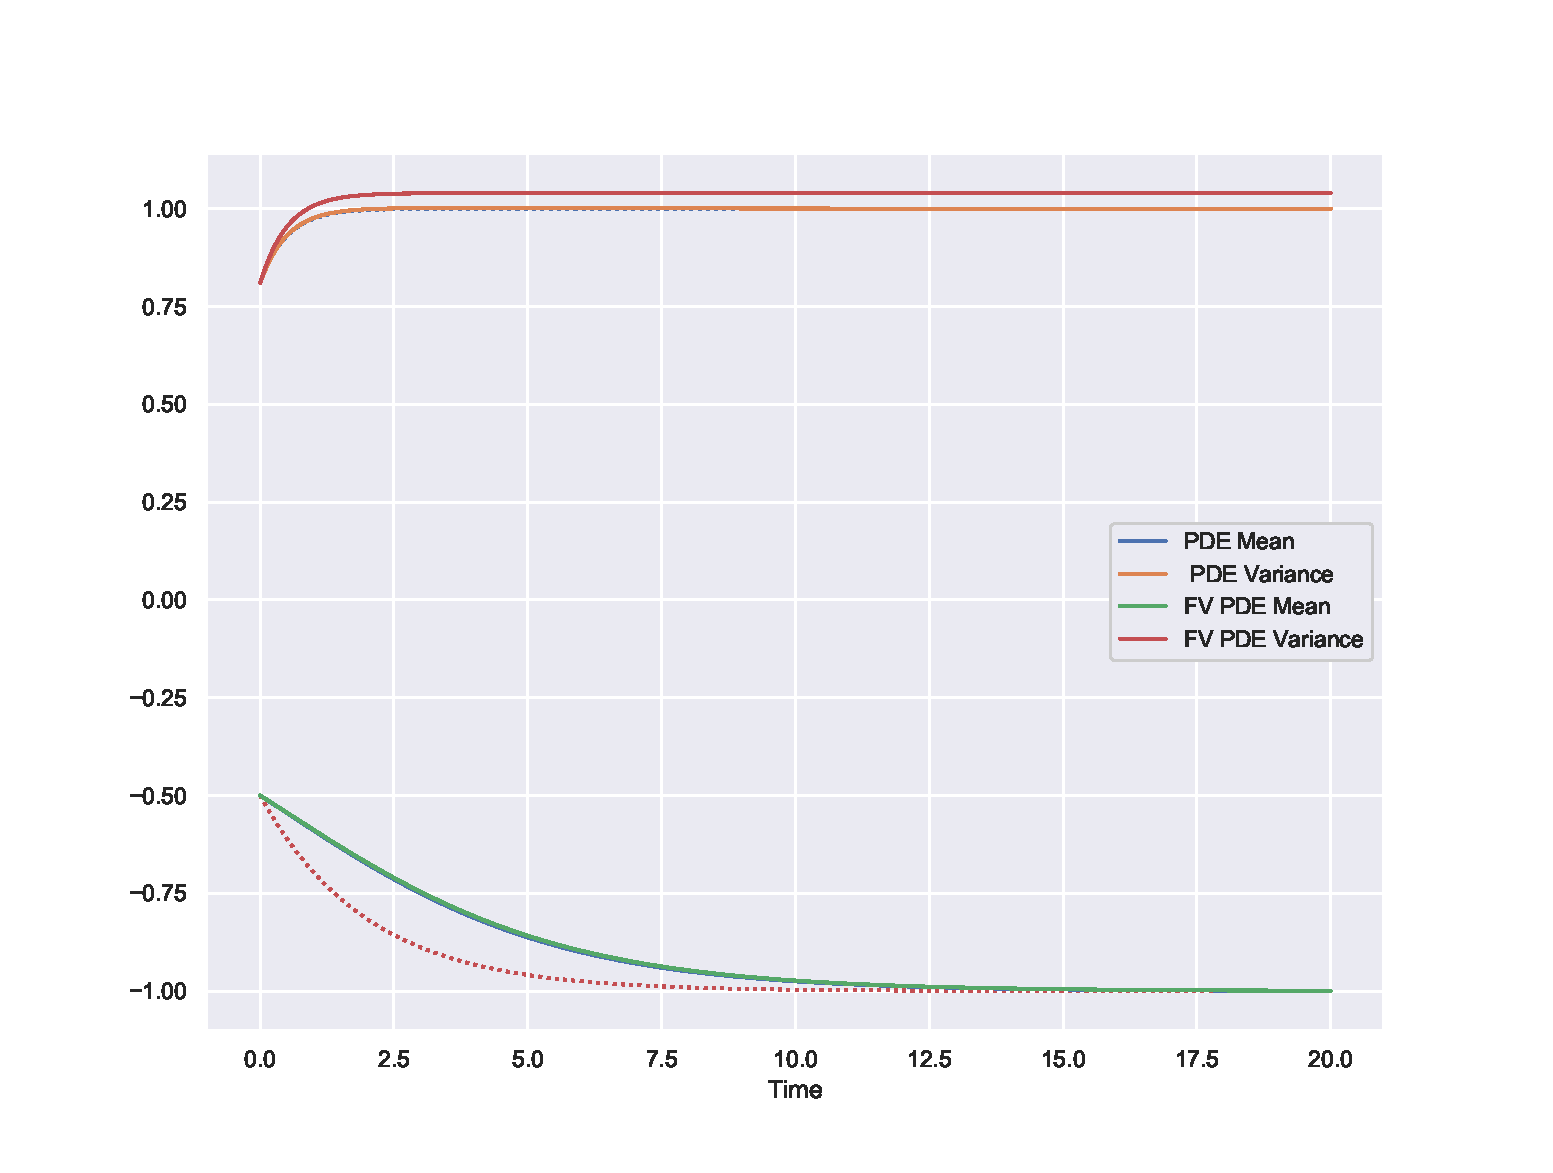
\includegraphics[width=0.8\linewidth]{Figures/kinmodelmomvar}
        \caption[Convergence of Moments for Kinetic Model]{For Gaussian initial data with mean -0.5 and variance 0.81, the schemes both converge with a time step of $\Dt =0.001$ and $\Dv = 0.05$. For the mean, the solvers are almost indistinguishable. The time step must be small so the FTCS scheme within the finite volume solver is stable. Also note the overestimation of variance. Blue line shows the analytic stationary distribution.}
        \label{fig:kinmodelmomvar}
    \end{figure}

    \begin{figure}
        \centering
        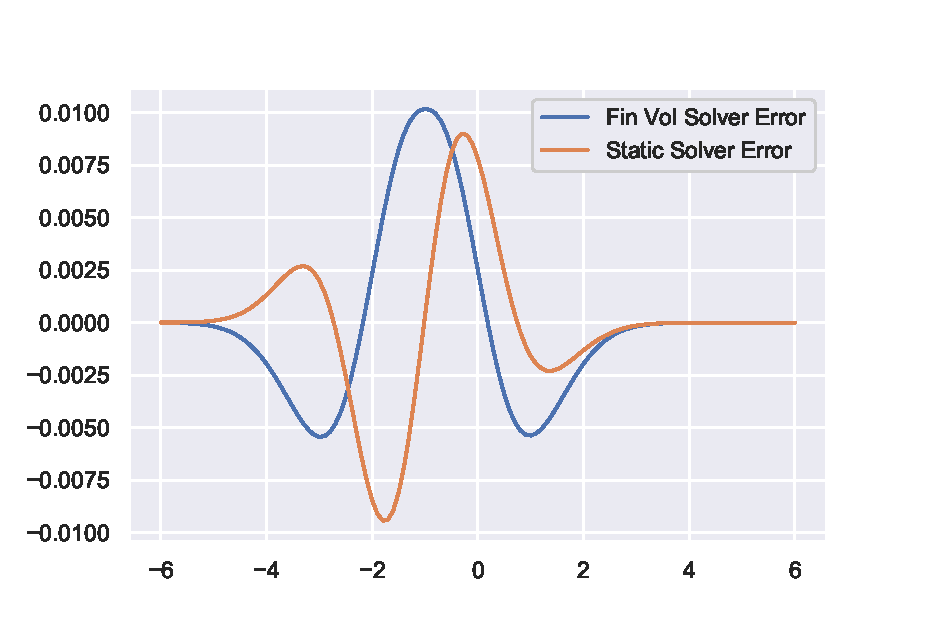
\includegraphics[width=0.7\linewidth]{Figures/homkinerror}
        \caption[Error of the Schemes]{Difference between approximate solution at $t=20$ and a Gaussian distribution with mean -1 and variance 1. Note the spatial bias in the `static' finite difference method has introduced a bias in the error. No such bias exists for the upwinding in the finite volume case.}
        \label{fig:homkinerror}
    \end{figure}
\subsection{Space-Heterogeneous Particle Model}\label{sec:hetkin}
    The next step is to reintroduce the spatial heterogeneity in the particle system. Recall the full particle model is given by
            \begin{equation}\begin{cases}
    \dif x^{i,N}_t = v^{i,N}_t\dif t\\
    \dif v^{i,N}_t = -v^{i,N}_t\dif t + G\left(\frac{\frac{1}{N}\sum_{j=1}^N \phi(x_t^{i,N} - x_t^{j,N})v^{j,N}_t  }{\frac{1}{N}\sum_{j=1}^N \phi(x_t^{i,N} - x_t^{j,N})}\right)\dif t + \sqrt{2\sigma} \dif W^i_t 
    \end{cases}, \qquad  i = 1,\dots,N.\tag{\ref{eq:fullparticle}}
    \end{equation} 
    Letting $\phi\equiv 1$ forces the interaction to be homogeneous in space, however there is now the movement of particles in space given by the first equation. The numerical simulations reflect what the analysis showed: particles will spread from their initial distribution until they are uniform in space, and average velocity converges to $-1, 0, +1$ depending on the sign of the mean of the initial data, see Figure \ref{fig:hetjointplot}. As in the space-homogeneous case, it is possible (and certain, if the system is allowed to run long enough) that the particles randomly switch from clockwise to counterclockwise movement. The animation \texttt{switch.mp4} shows exactly this behaviour.
    \begin{figure}
        \centering
        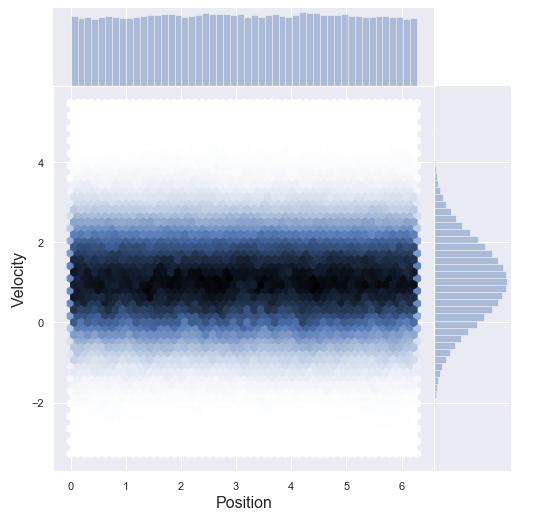
\includegraphics[width=0.7\linewidth]{Figures/hetjointplot}
        \caption[Joint Plot showing marginals of space-heterogeneous particle model]{Hex plot of 100 particles' positions and velocities up to $T=200$. This shows very clearly the uniformity in position and Gaussian distribution in velocity.}
        \label{fig:hetjointplot}
    \end{figure}

    \begin{figure}
        \centering
        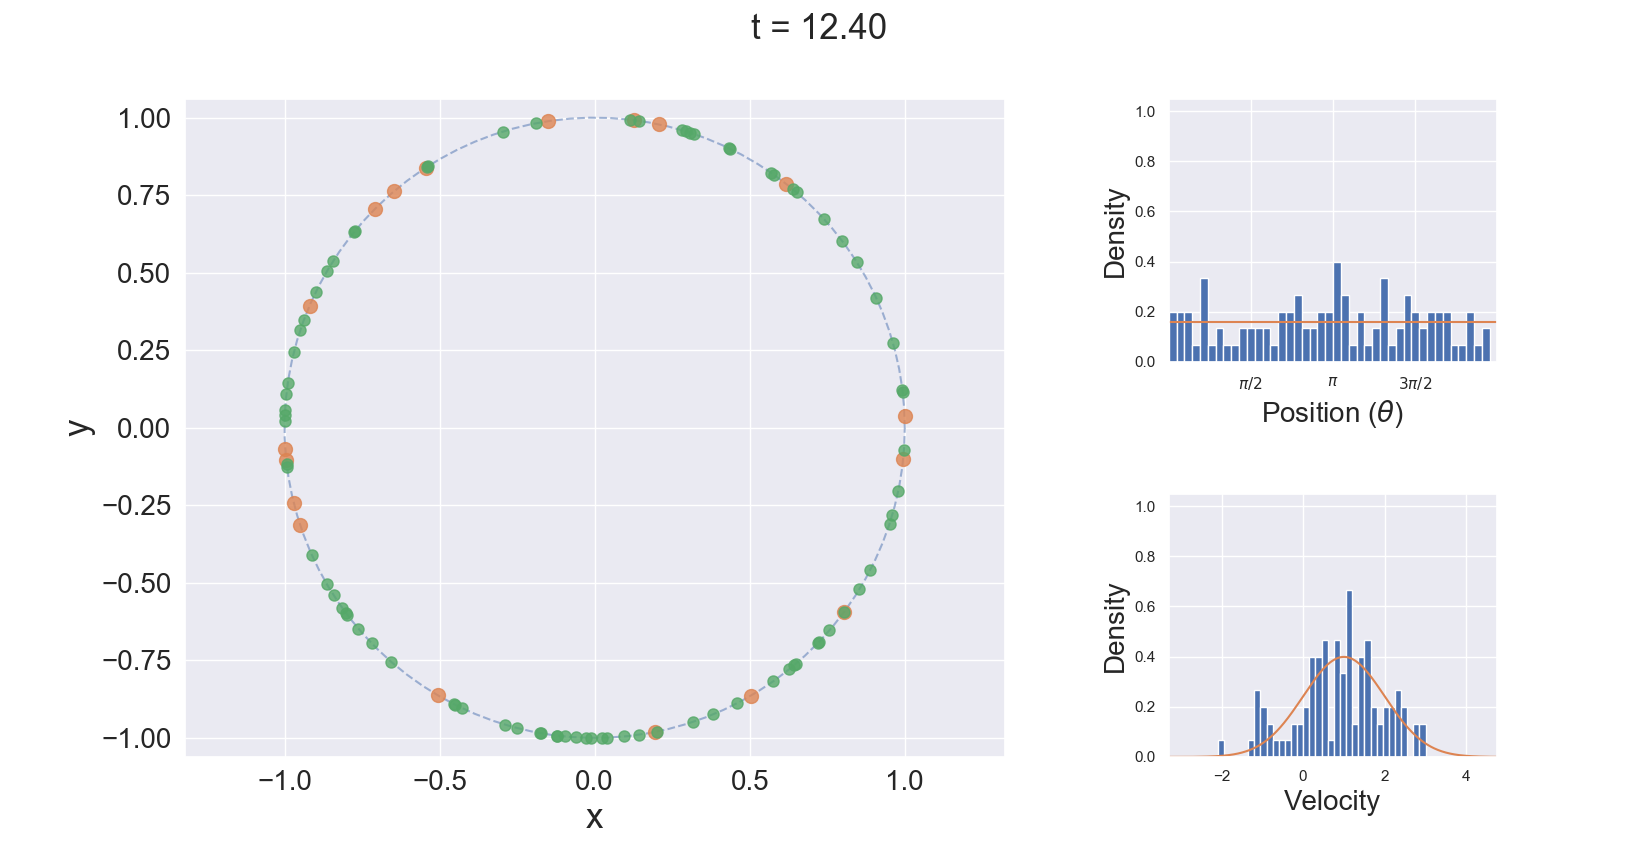
\includegraphics[width=\linewidth]{Figures/hetParticle}
        \caption[Particles on the torus]{Particle model with position variable included. Green circles indicate those travelling with positive velocity, orange shows negative velocity. This is again visual confirmation of what the analysis predicted for $\phi=1$.}
        \label{fig:hetparticle}
    \end{figure}
        
    \section{Discussion}\label{sec:discussion}
          +++

    \bibliographystyle{abbrv}
    \bibliography{whales.bib}
    \appendix
    \section{Implementation}\label{app:code}
    All the numerical schemes described above were implemented in Python 3. Before doing this project I had very little knowledge of Python beyond the basics, and a passing knowledge of MATLAB. As part of this project I have written a Python package to solve the toy problems, as well as the one-dimensional kinetic model and particle system. There is also a set of functions designed to produce animations and plots of the solutions. All of these are available and described further at 
    \begin{center}\url{https://github.com/Tom271/InteractingParticleSystems}\end{center}
    \texttt{Project Supplement.ipynb} shows the basic use of all the methods and how to produce plots and animations of the solution. The algorithms and functions themselves lie in the \texttt{src} folder as \texttt{.py} files, meaning they can be downloaded and used without Jupyter being installed.
 
    \section{Thomas Algorithm}\label{app:thomas}
    
\end{document}